%=========================================================================
% (c) Michal Bidlo, Bohuslav Křena, 2008
\todo{shrnuti kazde kapitoly!}
\todo{ukazka trajektorie spatneho genomu}
\todo{vlna!}

\chapter{Úvod}
Vygenerovano: \DTMnow

% vycistit kody
% zautomatizovat dokonceni behu, tj. vygenerovat vsechny zajimave a potrebne veci
% rucni skript jen po dokoneceni vsech behu a vyplivnuti nejakych statistik

%roztahnout uvod

%    - posledni odstavec zalozit na vysledcich a pridat odkaz na LGP knihu

%krabicov7 graf = box plot
%vysvetlit grafy

%cd: zdrojaky, uzivatelsky manual, jak nainstalovat a spustit aplikaci!
%po odevzdani se sejit s oponentem a zive mu to predvest.

%k lGP pripsat vice a dat priklady

%pro ucely teto rpace se vyzuiva koncept LGP, ktery je dale popsany v kapitole 4

%o hornbym asi 2 strany - napsat stranu o praci hornbyho a popsat inspiraci + obrazky, ktere hornby vyvinul

%pridat povidani k vysledkum
%obrazky vysledku dat na jednu stranu aby zabraly co nejmin mista


Robotika představuje v současné době velmi aktuální oblast aplikace výpočetní techniky, jejímž cílem je řízení nejrůznějších
elektromechanických systémů.
Uplatnění nacházejí roboti zejména v průmyslu, kde usnadňují a zefektivňují namáhavou a
opakující se práci člověku, ale také je populární oblast autonomních robotů používaných např. pro operace v těžko přístupných
nebo nebezpečných místech (např.ponorky, podpora záchranářům apod.).
Jedním ze zásadních problémů konstrukce robotů obecně je návrh jejich efektivního řízení ve vztahu ke konkrétnímu typu robota a podmínkám jeho nasazení~\cite{Bongard2013}.

Pro tyto potřeby je vhodné mít k dispozici prostředky, které nám umožní rychle a levně prototypovat různé koncepty řízení
robotů.
Jednou z možností, jak řadiče robotů navrhovat, je použití evolučních algoritmů.
Využití evolučních algoritmů osvobozuje konstruktéry od řešení malých detailů při návrhu kontroléru robota a v mnoha případech může evoluce nalézt řešení, které by lidského konstruktéra nenapadlo.

Řízení robota je ovšem možné realizovat mnoha způsoby, např. umělými neuronovými sítěmi~\cite{Reil2002}, konenčnými automaty~\cite{Hodgins1996} nebo i programy v imperativním jazyce~\cite{Wolff2007}.
V závislosti na vybrané metodě řízení robota jsou k dispozici různé alogritmy a automatizované nástroje pro nalezení konfigurace zvoleného způsobu řízení, které bude mít za následek požadované chování robota.
Touto konfigurací může být např. váhy neuronové sítě, definice konečného automatu nebo sekvence příkazů imperativního jazyka.
Právě řízením robota programy napsanými v imperativním jazyce (byť jednoduchém) se zabývá tato práce, ve které jsou použity evoluční algoritmy pro automatizované hledání vhodného řízení robota.

Cílem této práce je návrh a implementace nástroje pro automatizované hledání vhodného kontroléru robotického modelu pro průchod prostorem po dané trajektorii.
Pro návrh vhodného programu je použita technika zjednodušeného Lineárního Genetického Programování~\cite{Brameier2010}.
Pro simulaci pohybu robotického modelu byl použit simulátor Mujoco~\cite{Todorov2012}.
Účinnost softwarového řízení je experimentálně doložena s použitím dvou robotických modelů na dvou trajektoriích.

%%%%%%%%%%%%%%%%%%%%%%%%%%%%%%%%%%%%%%%%%%%%%%%%%%%%%%%%%%%%%%%%%%%%%%%%%%%%%%%%%%%%%%%%%%%%%%%%%%%%%%%%%%%%%%%%%%%%%%%%%%%%%%%%%%%%%%%%%%%%%%%%%%%%%%%%%%%%%%%%%%%%%%%%%%%
%%%%%%%%%%%%%%%%%%%%%%%%%%%%%%%%%%%%%%%%%%%%%%%%%%%%%%%%%%%%%%%%%%%%%%%%%%%%%%%%%%%%%%%%%%%%%%%%%%%%%%%%%%%%%%%%%%%%%%%%%%%%%%%%%%%%%%%%%%%%%%%%%%%%%%%%%%%%%%%%%%%%%%%%%%%
%%%%%%%%%%%%%%%%%%%%%%%%%%%%%%%%%%%%%%%%%%%%%%%%%%%%%%%%%%%%%%%%%%%%%%%%%%%%%%%%%%%%%%%%%%%%%%%%%%%%%%%%%%%%%%%%%%%%%%%%%%%%%%%%%%%%%%%%%%%%%%%%%%%%%%%%%%%%%%%%%%%%%%%%%%%


\chapter{Evoluční algoritmy}
V této kapitole si nejpreve v sekci~\ref{sec:koncept_ea} představíme základní koncept evolučních algoritmů.
Poté následuje v sekci~\ref{sec:gp} stručný úvod ke Genetickému Programování (GP), na který naváže sekce~\ref{sec:lgp} o Lineárním Genetickém Programováním (LGP).

\section{Koncept evolunčích algoritmů}
\label{sec:koncept_ea}
Informace v této sekci vycházejí z~\cite{Eiben2015}.

Evoluční algoritmy (EA) jsou inspirovány přírodními evolučními procesy a Darwinovou teorií evoluce.
EA se využívají ke stochastickému prohledávání stavového prostoru.
EA, narozdíl od jiných metod, pracují s celou populací kandidátních řešení (jedinců), které se vyvíjí paralelně.
Každý jedinec v populaci v sobě nese zakódovanou informaci o konktrétním řešení, kterou nazýváme genotyp.
Genotyp se poté dekóduje na fenotyp, který už reprezentuje řešení daného problému.

Myšlenku EA můžeme popsat následovně.
Máme populaci jedinců, kteří jsou všichni umístěni ve společném prostředí, ve kterém soutěží o zdroje.
To má za následek přirozený výběr jedinců, který se projevuje tak, že horší jedinci mají menší pravděpodobnost reprodukce, než-li ti lepší.
Tímto se přirozeně zvyšuje kvalita populace.
Reprodukce probíhá dvojím způsobem, a to křížením a mutací.
Křížení pracuje se dvěmi rodiči a má za následek vytvoření dvou potomků, kteří vznikají kombinací genotypu obou rodičů.
Mutace pracuje nad jedním rodičem a produkuje jednoho potomka, který má narozdíl od svého ročiče lehce pozměněný genotyp.

Činnost obecného EA můžeme vidět na algoritmu~\ref{alg:EA_alg}:


\begin{algorithm}[H]
    inicializuj populaci náhodně vygenerovanými jedinci\;
    vyhodnoť všechny jedince\;
    \While{(není splněna ukončující podmínka)}{
    vyber rodiče\;
    aplikuj křížení na dvojice rodičů\;
    mutuj potomky\;
    vyhodnoť kvalitu potomků\;
    vyber jedince do další generace\;
    }
    \caption{Obecný evoluční algoritmus}
    \label{alg:EA_alg}
\end{algorithm}

\subsection{Reprezentace}
Při návrhu řešení problému je často nutné abstrahovat reálný svět tak, aby jsme vytvořili prostředí, ve terém budou existovat kandidátní řešení a ve kterém budou tato řešení vyhodnocována.
Kandidátní řešení problému nazýváme fenotypy.
Zakódované fenotypy nazýváme genotypy.
Termín reprezentace se používá ve dvou kontextech.
V prvním kontextu specifikuje mapování z fenotypu na genotyp a je synonymem pro kódování.
V druhé kontextu označuje spíše strukturu prostoru genotypů.

\subsection{Fitness funkce}
Úlohou fitnes funkce je reprezentování požadavků, které by populace měla splňovat.
Tvoří základ pro funkci selekčních operátorů.
Můžeme mluvit o zobrazení z jedince v prostoru genotypů na reálné, nebo celé, číslo.
Z technického hlediska se jedná o funkci, která měří míru kvality genotypu a přiřazuje mu tzv. fitness.
Výpočet fitness funkce zahrnuje dekódování genotypu na fenotyp a následné vyhodnocení fenotypu, jako kandidátního řešení pro daný problém.

\subsection{Populace}
Úlohou populace je obsahovat množinu kandidátních řešení --- jedná se o multimnožinu jedinců.
Populace je struktura, která podléhá evoluci, zatímco jedinci jsou statické struktury.
Definice populace se může omezit pouze na její velikost, ale existují i specializované evoluční algoritmy, které pracují i s rozložením jedinců v prostoru.


\subsection{Selekce}
Operátor selekce slouží k výběru rodičů pro křížení na základě jejich kvality.
Tento operátor je nejšastěji založen na náhodě a to tak, že kvalitnější řešení jsou vybárána s větší pravděpodností.
Změnou parametrů selekce nastavujeme tzv. selekční tlak, který ovlivňuje, do jaké míry jsou upřednostňováni lepší jedinci.

Jako představitele selekce si můžeme uvést ruletovou selekci a selekci turnajem.
\todo{ruleta}

Selekce turnajem, narozdíl od ruletové selekce nevyžaduje znalost celé populace a přepočítávání fitness hodnot.
Selekce turnajem ani nevyžaduje, aby vyhodnocení fitness funkcí bylo kvantifikované, ale pro jeho funkci stačí, aby byla mezi jedinci definována operace uspořádání.
Díky toho je tato metoda nenáročná na implementaci a na výpočetní čas.
Základní alogoritmus selekce turnajem můžeme vidět na algoritmu~\ref{alg:EA_turnaj}.

\begin{algorithm}[H]
    // Chceme vytvořit mating pool velikosti $\lambda$ jedinců\;
    \While{(dokud mating pool neobsahuje $\lambda$ jedinců)}{
    Náhodně vyber $k$ jedinců\;
    Porovnej mezi sebou těchto $k$ jedinců a vyber z nich nejlepšího jedince $i$\;
    Vlož jedince $i$ do mating pool
    }
    \caption{Selekce turnajem}
    \label{alg:EA_turnaj}
\end{algorithm}

Úpravou parametru $k$ se nastavuje selekční tlak --- čím větší je parametr, tím více jedinců je vybráno pro porovnání a to má za následek vyšší selekční tlak.

\subsection{Křížení}
Operátor křížení slouží ke spojení částí genotypů rodičů a tím dochází k vytvoření nových jedinců.
Operátor je většinou aplikován pouze s určitou pravděpodobností $p_r$.
Nejčastěji se používá křížení pracující se dvěmi rodiči.
Výběr, jeké části ze kterého rodiče budou vybrány, je založen na náhodě.
Myšlenka za použitím křížení je následující.
Zkombinováním rodičů, kteří mají odlišné, ale vhodné vlasnosti, může vzniknout jedinec, který tyto vlastnosti v sobě kombinuje a dosahuje tak vyšší kvality.

Jako představitele si můžeme uvést jednobodové a uniformní křížení.

Jednobodové křížení bylo původně představeno J. H. Hollandem v \todo{220} a jeho funkce je následující.
Vygeneruje se náhodné číslo $r$ z intervalu $\langle 1, L-1\rangle$, kde L je délka genomu.
Poté se genomy rozdelí v tomto bodě $r$ na počáteční a koncovou část a noví jedinci vznikají záměnou těchto koncových částí, viz obrázek~\ref{fig:jednobodove_krizeni}.

\begin{figure}[h]
    \centering
    {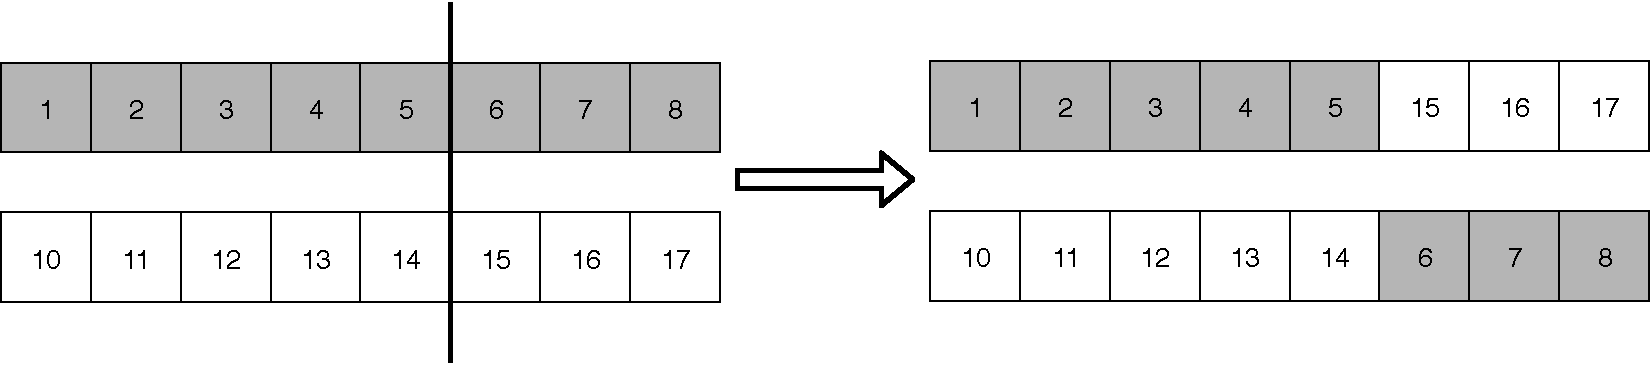
\includegraphics[width=30em]{obrazky/jedobodove_krizeni.pdf}}
    \caption{
    Jednobodové křížení
    }
    \label{fig:jednobodove_krizeni}
\end{figure}

Uniformní křížení bylo představeno v \todo{422} a pracuje následovně.
Pro každý gen se vygeneruje náhodné číslo $r$ z rovnoměrného rozložení na intervalu $\langle 0, 1\rangle$.
Číslo $r$ se poté porovná s parametrem $p$, který bývá obvykle roven 0.5, a pokud je $r < p$, tak se použije gen z prvního rodiče, jinak ze druhého.
Druhý potomek je vytvořen z genů, které nebyly vybrány do prvního potomka, viz obrázek~\ref{fig:uniformni_krizeni}

\begin{figure}[h]
    \centering
    {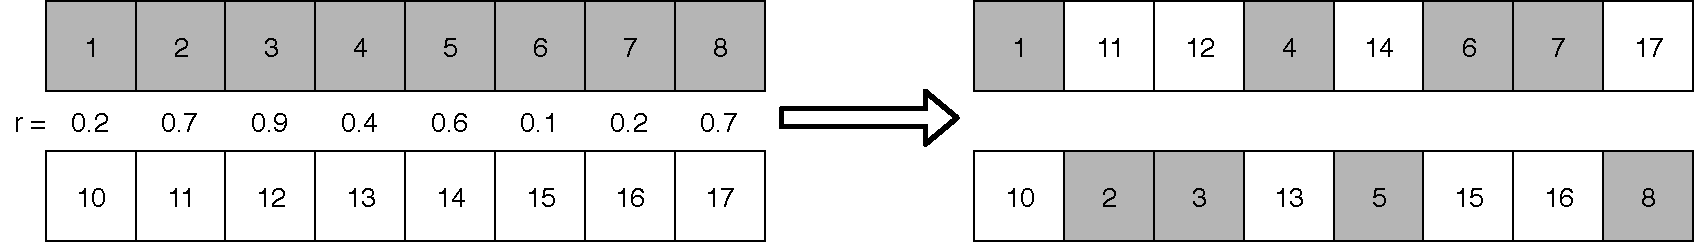
\includegraphics[width=30em]{obrazky/uniformni_krizeni.pdf}}
    \caption{
    Uniformní křížení
    }
    \label{fig:uniformni_krizeni}
\end{figure}


\subsection{Mutace}
Operátor mutace se aplikuje na jendoho rodiče a jeho výsledkem je jeden potomek.
Cílem mutace je provést malou změnu genotypu.
Operátor je většinou aplikován pouze s určitou pravděpodobností $p_m$ a jeho implementace je závislá na použité reprezentaci.


Např. pro reprezentace využívající celá čísla, existují 2 záladní přístupy, které mutují každý gen s pravděpodobností $p_m$.
Prvním přístupem je úplné nahrazení aktuální hodnoty genu novou hodnotou.
Tato varianta je vhodná, pokud mezi hodnotami neexistuje relace uspořádání.
Druhým způsobem je malá změna aktuální hodnoty, při které se k hodnotě genu přičte nebo odečte náhodně vygenerované malé číslo.
Tato varianta je vhodná, jsou-li hodnoty genomu např. parametry systému nebo funkce.

\subsection{Ukončovací podmínka}
Ukončovací podmínka určuje, kdy se zastaví evoluce aktuální populace.
K tomuto je možné využít: dosažení předem dané fitness hodnoty, spotřebování určeného strojového času, provedení určeného počtu vyhodnocení fitness funkce, ukončení v případě, že se populace dostatečně rychle nezlepšuje nebo že pokud dojde ke snížení diverzity populace po daný limit.

\section{Genetické programování}
\label{sec:gp}

Informace v této sekci vycházejí z~\cite{Koza1992}.

Genetické programování (GP) se zabývá evolucí programu, který je reprezenotván stromovou strukturou.
Programy v GP jsou složeny z funkcí, které ve stromové struktuře odpovídají uzlům, a terminálů, které odpovídají listům.

Vyvíjené programy jsou typicky vyhodnocovány nad sadou vstupů, tzv. fitness cases, u kterých jsou známy požadované výstupy programu.
Výsledná fitness programu se pak může počítat jako suma nebo průměr výsledků z každého "fitness case".

V GA je nejdůležitějším operátorem křížení.
Křížení pracuje na základě výměny náhodně vybraných podstromů z rodičů.
Toto křžení se skládá z několika kroků.
Prvním krokem je výběr rodičů.
Druhý krok je zvolení náhodného uzlu v každém z rodičů.
Tento uzel bude kořenový uzel pro podstromy, které se budou později mezi rodiči vyměňovat.
Třetím krokem je vyjmutí podstromu z obou rodičů, jejichž kořenovým uzlem je uzel, který byl vybrán v předchozím kroku.
Následuje vytvoření obou potomků.
První potomek vznikne tak, že se do stromu prvního rodiče, do místa dříve vybraného uzlu, vloží podstrom z druhého rodiče.
Druhý jedinec vzniká obdobným způsobem, viz. obrázek~\ref{fig:GP_krizeni}.

\begin{figure}[h]
    \centering
    {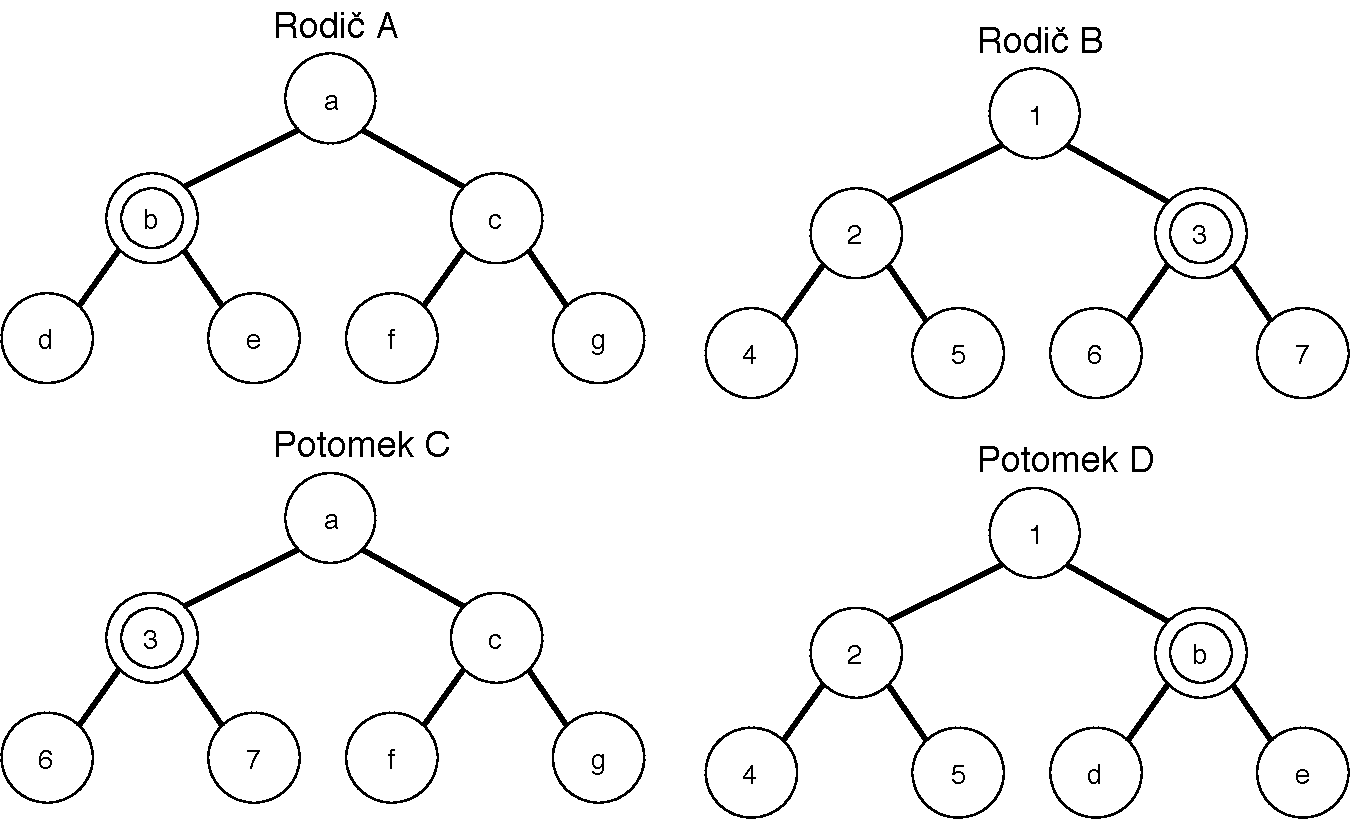
\includegraphics[width=30em]{obrazky/gp_krizeni.pdf}}
    \caption{
    Křížení v GP.
    Na tomto obrázku je zachycena situace, kdy je v každém z rodičů A a B náhodně vybrán uzel(vyznačen dvojitě).
    Tyto uzly a jejich podstromy jsou poté zaměněny a vznikají tak potomci C a D.
    }
    \label{fig:GP_krizeni}
\end{figure}

Velikost programu, definována jako výška stromu, je omezena aby se předešlo velmi velkým programům.
Pokud by potomek po křížení přesáhl tuto velikost, nebude vložen do nové generace - místo něj se do nové generace zkopíruje jeden z jeho rodičů.

Mutace v GA hraje menší roli a provádí drobné změny struktur v populaci.
Mutace sestává z několika kroků:
První krok je zvolení náhodného uzlu ve struktuře.
Tento uzel může být vnitřní (funkce) i vnější (terminál).
Druhým krokem je odstranění tohoto uzlu is celým podstromem, který je k němu připojený.
Posledním krokem je vygenerování náhodného podstromu, který se poté připojí na místo odstraněného uzlu.
Tato operace je řízena parametrem který říká, jakou výšku bude mít vygenerovaný podstrom.
Speciálním případem mutace je operace, která vloží jeden terminál do náhodně vybraného uzlu ve stromu.

\section{Lineární genetické programování}
\label{sec:lgp}

V této práci se používá přístup inspirovaný Lineárním genetickým programováním (LGP), které si stručně popíšeme v této sekci, krerá vychází z~\cite{Brameier2010}.

LGP je varianta GP, popsaného v kapitole~\ref{sec:gp}, ve které jsou programy reprezentovány jako posloupnost instrukcí strojového kódu nebo příkazů vhodného imperativního jazyka.
Obecně jsou data, zpracovávaná pomocí programu LGP, uchovávána v registrech, které jsou součástí interpretu LGP.

Interpret má k dispozici sadu registrů, jejichž počet je definován uživatelem.
Tyto registry se dělí na vstupní, výstupní a pracovní registry.
Vstupní registry obsahují vstupní data, se kterými je program spouštěn.
Pracovní registry jsou určeny pro uložení mezivýsledků výpočtů a jsou před spuštěním programu inicializovány vhodnou konstantou, např. 1.
Jeden nebo více vstupních nebo pracovních registrů může být označeno jako výstupní registr, ze kterého se poté po zkončení programu čte výsledek.

Programy v LGP mohou být také vykonávány bez interpretu, a to tak, že se převedou do programu v jazyce C.
Ukázkový program v jazyce C můžeme vidět na obrázku \todo{XXX}

Imperativní instrukce obsahuje operaci, která pracuje nad zdrojovými registry, a přiřazení výsledku do cílového registru.

Instrukční sada definuje programovací jazyk, ve kterém jsou vyvíjené programy napsány.
LGP systém je založen na dvou základních typech instrukcí: operace a podmíněné větvení.
Příklady operací mohou být: různé aritmetické operace, exponenciální funkce, trigonometrické funkce, nebo booleovské operace.

V LGP je nutné zajistit, aby byly vytvářený pouze programy, které jsou validní.
Gentické operátory mutace a křížení proto musí zachovat syntaktickou správnost nově vytvořených programů.
Toho lze zajistit například tak, že bod křížení nemůže být určen urvnitř instrukce, nebo při aplikováni operátoru mutace zakážeme záměnu operátoru instrukce za registr.
Pro zajištění sémantické správnosti je nutné ošetřit všechny operátory a funkce, které nejsou definovány pro všechny možné hodnoty, tak aby pro nedefinovaný výstup vracely konstantu, např. velké celé číslo.

Schopnost genetického programování nalézt řešení velmi závisí na zvolené instrukční sadě.
Kompletní instrukční sada je taková, která obsahuje všechny prvky, které jsou potřebné k vytvoření optimálního řešení za předpokladu, že je počet registrů a rozsah použitých konstant dostatečný.
Na druhou starnu, rozměr stavového prostoru, který obsahuje všechny programy, které je možné sestavit z dostupných instrukcí, roste exponenciálně s počtem instrukcí a registrů.

Na programu \ref{code:lgp_c} v jazyce C si ukážeme průběh vykonávání programu pro výpočet průměru 2 čísel.
Tento program má k dispozici výstupní registr r[0], ve kterém bude uložen výsledek, dva vstupní registry r[1] a r[2], které obsahují vstupy programu a jeden pracovní registr r[3].
Před spuštěním programu jsou do vstupních registrů nakopírovány hodnoty a pracovní registr je inicializován na hodnotu 1.
První instrukcí programu je sečtení dvou vstupních registrů a uložení výsledku do pracovního registru.
Tento pracovní registr je poté využit jako operand pro instrukci dělení, která uloží výsledek do výstupního registru r[0].


\lstset{language=C,caption={LGP program v C pro sečtení 3 čísel},label=code:lgp_c}

\begin{lstlisting}
    double r[4];

    void lgp(r)
    {
        r[3] = r[1] + r[2];
        r[0] = r[3] / 2;
    }
\end{lstlisting}

%%%%%%%%%%%%%%%%%%%%%%%%%%%%%%%%%%%%%%%%%%%%%%%%%%%%%%%%%%%%%%%%%%%%%%%%%%%%%%%%%%%%%%%%%%%%%%%%%%%%%%%%%%%%%%%%%%%%%%%%%%%%%%%%%%%%%%%%%%%%%%%%%%%%%%%%%%%%%%%%%%%%%%%%%%%
%%%%%%%%%%%%%%%%%%%%%%%%%%%%%%%%%%%%%%%%%%%%%%%%%%%%%%%%%%%%%%%%%%%%%%%%%%%%%%%%%%%%%%%%%%%%%%%%%%%%%%%%%%%%%%%%%%%%%%%%%%%%%%%%%%%%%%%%%%%%%%%%%%%%%%%%%%%%%%%%%%%%%%%%%%%
%%%%%%%%%%%%%%%%%%%%%%%%%%%%%%%%%%%%%%%%%%%%%%%%%%%%%%%%%%%%%%%%%%%%%%%%%%%%%%%%%%%%%%%%%%%%%%%%%%%%%%%%%%%%%%%%%%%%%%%%%%%%%%%%%%%%%%%%%%%%%%%%%%%%%%%%%%%%%%%%%%%%%%%%%%%

\chapter{Zkoumání pohyblivých objektů}
\todo{3. Zkoumani pohyblivych objektu (zakladni myslenky shrnte s inspiraci v
clancich G. Hornbyho. ~3 strany. Zamerte se v zaverecne podsekci na
popis objektu, ktere budete mit v BP.}



Tato práce a pohyblivé struktury, se kterými se pracuje, je inspirována dizertací G. Hornbyho.
G. Hornby ve své práci využíval generativné reprezentace pro development struktury i kontroléru robotů.
[todo obrazky nekterych robotu hornbyho ]
Kotroléry byly realizovány pomocí oscilátorů nebo neuronových sítí.

%Wolff a Wahde použili LGP pro návrh kontroléru modelu humanoidního robota, který měl v simulovaném prostředí chodit a následovat zvukové signály.

%[todo: overit ] Wolff a Wahle použili LGP s čísly s plovoucí řádovou čárkou, aritmetické, matematický instrukce a větvení.
%[todo: overit ] Jejich kontrolér měl informace o natočení všech kloubů modelu a na základě těchto informací programy řídily model robota.

\section{Použité modely}
Níže si popíšeme dva modely robotů, se kterými byly provedeny experimenty.

První model, zvaný trojnožka, je vidět na obrázku~\ref{fig:trojnozka}
Robot má 3 nohy, každá z nich je spojena s jádrem robota kloubem, který se otáčí v jedné ose.
Rozsah pohybu těchto kloubů je omezen na 50 stupňů.
Model robota má v horní části v místě kloubů umístěny kontaktní body.
Tyto body slouží k detekci převrácení robota (kolizi ze zemí).

\begin{figure}[h]
    \centering
    {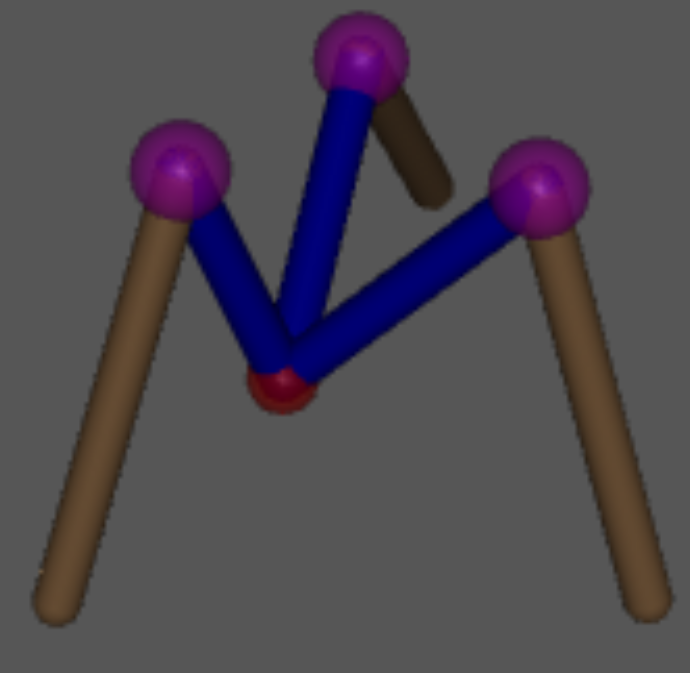
\includegraphics[width=15em]{obrazky/trojnozka_detail.png}}
    \caption{
    Model robota zvaný trojnožka.
    Tento model je složen z jádra robota (modře) a 3 nohou (hnědě).
    Každá z nohou je s jádrem spojena kloubem, který se otáčí pouze v jedné ose a je umístěn pod fialovou koulí.
    Tyto fialové koule slouží k detekci převrácení robota.
    Ve středu robota je bod zvaný hlava (červeně).
    }
    \label{fig:trojnozka}
\end{figure}


Druhý robot, zvaný mravenec, je vidět na obrázku~\ref{fig:mravenec}
Robot má 3 páry nohou, které jsou všechny připojeny k tělu robota.
Rozsah pohybu kloubů, které rotují kolem horizontální osy a spojují tělo robota s jeho nohou, je omezen na 100 stupňů.
Rozsah kloubů, které rotují kolem svislé osy a spojují dvě části nohy, je omezen na 65 stupňů.


\begin{figure}[h]
    \centering
    {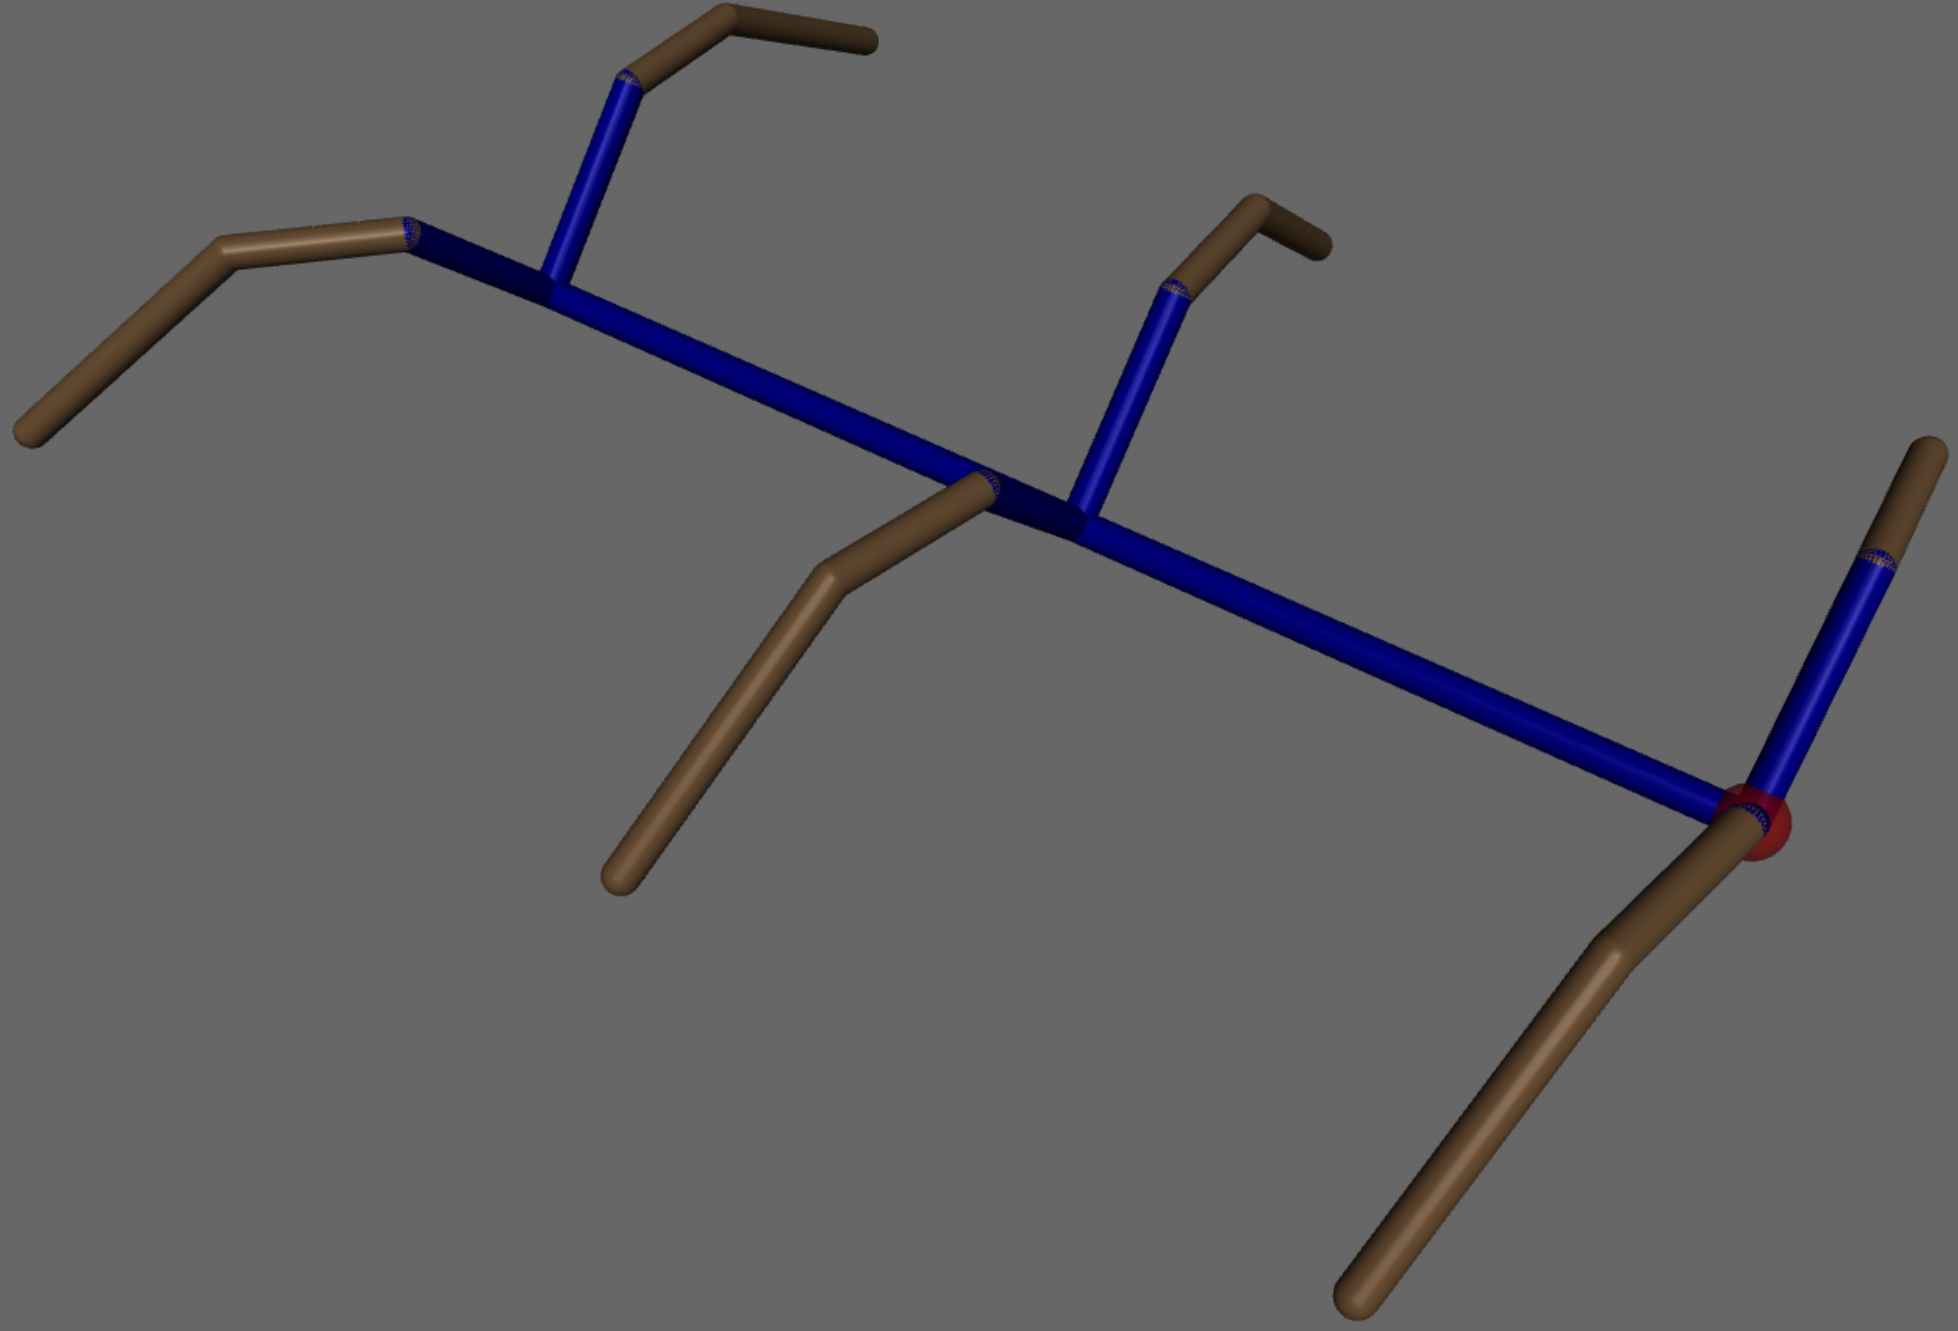
\includegraphics[width=30em]{obrazky/mravenec_detail.png}}
    \caption{
    Model robota zvaný mravenec.
    Tento model je složen z těla robota (modře) a 6-ti nohou (hnědě).
    V přední části robota je bod zvaný hlava (červeně).
    Každá noha je složena ze dvou pevných částí a jedoho kloubu.
    Tento kloub se pohybuje pouze ve svislé ose, tj. může zvedat a snižovat robota.
    Celá noha je připojena k tělu robota kloubem, který se pohybuje horizontálně, tj. slouží k odrážení.
    }
    \label{fig:mravenec}
\end{figure}

%%%%%%%%%%%%%%%%%%%%%%%%%%%%%%%%%%%%%%%%%%%%%%%%%%%%%%%%%%%%%%%%%%%%%%%%%%%%%%%%%%%%%%%%%%%%%%%%%%%%%%%%%%%%%%%%%%%%%%%%%%%%%%%%%%%%%%%%%%%%%%%%%%%%%%%%%%%%%%%%%%%%%%%%%%%
%%%%%%%%%%%%%%%%%%%%%%%%%%%%%%%%%%%%%%%%%%%%%%%%%%%%%%%%%%%%%%%%%%%%%%%%%%%%%%%%%%%%%%%%%%%%%%%%%%%%%%%%%%%%%%%%%%%%%%%%%%%%%%%%%%%%%%%%%%%%%%%%%%%%%%%%%%%%%%%%%%%%%%%%%%%
%%%%%%%%%%%%%%%%%%%%%%%%%%%%%%%%%%%%%%%%%%%%%%%%%%%%%%%%%%%%%%%%%%%%%%%%%%%%%%%%%%%%%%%%%%%%%%%%%%%%%%%%%%%%%%%%%%%%%%%%%%%%%%%%%%%%%%%%%%%%%%%%%%%%%%%%%%%%%%%%%%%%%%%%%%%

\chapter{Evoluční návrh pohyblivých objektů}
V této kapitole si nejdříve popíšeme způsob, jakým je realizováno řízení robota a poté instanci EA, která je v této práci použita.


\section{Relizace řízení modelu}
V simulátoru Mujoco je vytvořena scéna, která obsahuje model a množinu referenčních bodů, které svým pořadím a umístěním ve scéně definují trajektorii, kterou má modelu následovat.

\subsection{Interpret}
Program, který řídí model robota, je vykonáván v interpretu.
Interpret obsahuje vstupní, výstupní a konstantní registry.
Každý registr je indetifikovaný unikátním číslem, které se navýzá index.
Registry mohou obsahovat celočíselné hodnoty v rozsahu od -5 do 5.
Počty registrů jsou následující: 11 konstatních registrů s hodnotami od -5 do 5, 2 vstupní registry, a 3, nebo 12, výstupních registrů (pro každý kloub modelu jeden registr).
Interpret vykonává program, který je složen z instrukcí.

Je zde použit jen jeden druh instrukce, a to instukce s názvem COPY\@.
Tato instrukce má 2 parametry: zdrojový registr a cílový registr.
Výsledkem této instrukce je zkopírování hodnoty ze vstupního, nebo konstatního, registru do výstupního registru.
Interpret je schématikcy znázorněn na obrázku~\ref{fig:interpret}

\begin{figure}[h]
    \centering
    {
\includegraphics[width=30em]{obrazky/interpret.eps}}
    \caption{
    Schéma interpretu.
    Je zde znázorněna situace, ve které interpret vykonává instrukci z podprogramu main.
    Tato instrukce, s parametry 11 a 14 způsobí zkopírování hodnoty 3 ze vstupního registru s indexem 11 do výstupního registru s indexem 14.
    }
    \label{fig:interpret}
\end{figure}

V průběhu simulace je vykonáván program, který čte hodnoty ze vstupních registrů, které obsahují informaci o směru k dalšímu referenčnímu bodu, nebo konstantních registrů a zapisuje hodnoty do výstupních registrů, které se převádí na sílu, která je aplikována v jednotlivých kloubech.

\subsection{Podprogramy}

Pro účely experimentů se spirálovou trajektoríí byl navržen koncept podprogramů, který je popsán dále.
V experimentech s přímkovou trajektorií je z těchto podprogramů použit jen podprogram main.

Každý program, který reprezentuje kandidátní řešení, je pro vykonávání v průběhu simulace rozdělen na 3 podprogramy.
Tyto podprogramy se nazývají init, main a event.

Podprogram init se vykoná pouze na začátku simulace a všechny instrukce jsou provedeny v nulovém čase a poté je po 1 sekundě spuštěn podprogram main.
Účelem podprogramu init je nastavení počátečního natočení kloubů modelu.

Podprogram main je v průběhu simulace vykonáván v nekonečné smyčce.
Instrukce v tomto podprogramu se nevykonají všechny v nulovém čase, ale vyonávají se s periodou 0.3 sekundy.
Jedná se o nejdelší a nejdůležitější podprogram.

Podprogram event se vykoná v situaci, kdy se model přiblíží do určené vzdálenosti od referenčního bodu, avšak pro každý referenční bod pouze jednou.
Stejně jako u podprogramu init jsou instrukce provedeny v nulovém čase a poté je po 1 sekundě spuštěn podprogram main.
Účelem podprogramu event je změna natočení kloubů modelu jako příprava k pohybu k následujícímu referečnímu bodu.

\subsection{Hodnoty vstupních registrů}
Hodnoty, které se ukládájí do vstupních registrů, vychází z informace o směru k následujícímu referenčnímu bodu.
Informace o směru je opět vyjádřena číslem od -5 do 5 a vypočítává se následujícím mechanismem.

Prostor kolem modelu je rozdělen na 11 kruhových výsečí, kde každá výseč je ohodnocena číslem od -5 do 5, viz obrázek~\ref{fig:kruhove_vysece}.
Informace o směru je rovna ohodnocení výseče, ve které se nachází další referenční bod.
Tato informace je v nezměněné podobě vložena do prvního vstupního registru.
Do druhého registru je vložena hodnota s převráceným znaménkem.

\begin{figure}[h]
    \centering
    {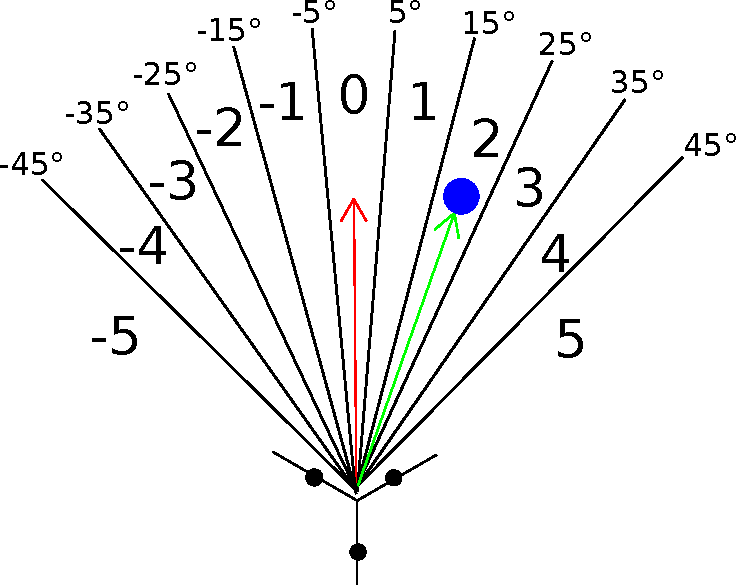
\includegraphics[width=20em]{obrazky/reference_direction_angles.pdf}}
    \caption{
    Způsob výpočtu hodnot vstupních registrů.
    Model (na obrázku dole) směřuje směrem nahoru a další referenční bod (modře) se nachází ve výseči ohodnocené číslem 2.
    Hodnoty vstupních registrů budou tedy čísla 2 a -2.
    }
    \label{fig:kruhove_vysece}
\end{figure}

\subsection{Výstupní registry}

Každý z výstupních registrů interpretu odpovídá jednomu kloubu modelu.
Hodnoty z výstupního registru jsou z interpretu čteny a převádí se na ovládací signály, které se předávají simulátoru.
Hodnota (ovládací signál) v sobě obsahuje dvě informace.
První z nich je dána znaménkem a určuje, kterým směrem bude aplikována síla v kloubu.
Druhá informace je dána velikostí hodnoty a určuje velikost této síly.


\subsection{Simulátor}
Simulátor Mujoco je dynamická knihovna napsaná v jazyce C.
Tato knihovna poskytuje řadu funkcí, které umožňují řídít běh simulace.
Tyto funkce se poté používají v uživatelském programu, ve kterém nutné z těchto funkcí sestavit algoritmus spojité simulace (ukázkové uživatelské programy jsou součástí distribuce simulátoru).
Uživatel má plnou kontrolu nad během simulace, a to tím, že volá knihovní funkci mj\_step(), která v simulaci pokročí definovaným krokem.
Ve smyčce algoritmu spojité simulace jsou vloženy funkce zajišťující běh interpretu, výpočet fitness funkce, mapování výstupních hodnot z interpretu na ovládací signály a získávání pozic objektů z dat simulace.
Ve zjednodušené formě je program znázorněn na algoritmu~\ref{alg:algoritmus_simulatoru}.

\todo{popsat, jak se tvori modely v xml jazyce?}

\begin{algorithm}[H]
    Načti model ze souboru\;
    Nastav čas simulace $t = 0$\;
    Vykonej celý program init\;
    \While{($t$ < délka simulace)}{
    Proveď další kroku simulace - mj\_step()\;
    \If{(došlo ke kolizi se zemí)}{
    Ukonči simulaci\;
    }
    Vypočti vstupní hodnoty interpretu\;
    Vykonej instrukci z programu main\;
    Použij výstupní hodnoty interpretu pro řízení modelu\;
    Zaznamenej vzdálenosti od jednotlivých referenčních bodů\;
    \If{(došlo k přiblížení k následujícímu referenčnímu bodu)} {
    Vykonej celý program event\;
    }
    Přičti k času $t$ časový krok simulace\;
    }
    Vypočti fitness hodnotu\;
    \caption{Algoritmus simulátoru}
    \label{alg:algoritmus_simulatoru}
\end{algorithm}

\section{Instance evolučního algoritmu}

\subsection{Reprezentace}
Použtá reprezentace pracuje s genomem fixní délky, která se liší pro každý model a experiment.
Tato délka bude uvedena u každého z experimentů v následující kapitole.
Tato reprezentace kóduje každou instrukci jako n-tici, ve které je prvním prvkem název instrukce a poté následují její argumenty.
Aktuálně jediná použitá instrukce je složena ze svého názvu (COPY, nebo i starší název SRE) a dvou celých čísel, které označují zdrojový a cílový registr.

Tato n-tice je použita jako hodnota jednoho genu \todo{alela?}.
Pro experimenty se spirálovou trajektori je celý genotyp pro účely křížení rozdělen na 3 části, které korespondují s podprogramy, viz obrázek~\ref{fig:genotyp}.

\begin{figure}[h]
    \centering
    {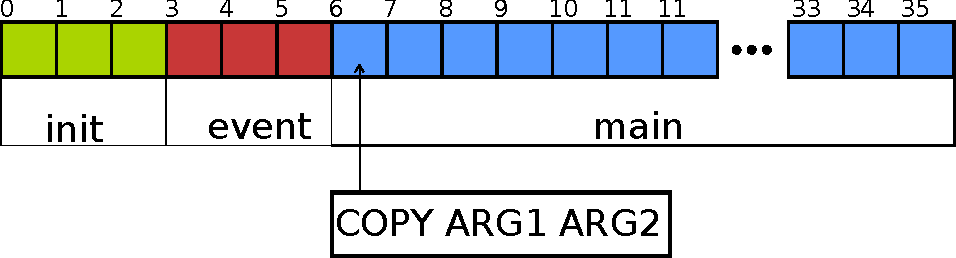
\includegraphics[width=30em]{obrazky/genotyp.pdf}}
    \caption{
    Rodzdělení genotypu na části pro podprogramy.
    Je zde znázorněn genotyp délky 36 genů, který je rozdělen po 3 genech pro podprogram init a event a 30 genů pro podprogram main.
    Je zde také znázorněna n-tice, která reprezentuje instrukci.
    }
    \label{fig:genotyp}
\end{figure}


\subsection{Fitness funkce}
Fitness hodnota programu se počítá následující způsobem.
V průběhu simulace se pro každý referenční bod $i$ zaznamenává nejmenší vzdálenost $D_i$ mezi tímto bodem a modelem.
$D_i = \min{F(R, P_i)}$, kde $F$ je funkce vypočítávající vzdálenost, $R$ je pozice modelu v prostoru, $P_i$ je pozice referenčního bodu v prostoru a $i=1, \cdots N$, kde $N$ je pocet referenčních bodů.

Po dokončení simulace je pro každý referenční bod je vypočteno skóre následujícím způsobem:
$$S_i=\left\{\begin{matrix}
                 t - D_i&\mbox{ pokud }D_{i}\leq t\\ 0 &\mbox{ jinak }
\end{matrix}\right.$$

Parametr $t$ je minimální vzdálenost, ve které musí být model od referenčního bodu, aby se skóre pro tento bod počítalo.
Výsledná fitness hodnota je poté vypočtena jako suma skóre pro všechny body:
$$f=\sum_{i=1}^{N}S_i$$

Na základe rozměru modelu a celé scény v simulátoru byla zvolena hodnota parametru $t = 40$.

\subsection{Populace a selekce}
Pro evoluci programů byla vybrána varianta steady-state algoritmu (algoritmus~\ref{alg:ss_algoritmus}) s velikostí populace 1000 nebo 400 jedinců.
Operátor selekce je implementován jako turnaj velikosti $k = 2$.
Nejlepší jedinec v aktuální populaci a jeho mutant jsou zkopírováni do následující populace.

\begin{algorithm}[H]
    \SetKwRepeat{Do}{do}{while}

    nastav čas t = 0\;
    inicializuj všechny chromozomy v P(t) náhodnými alelami\;
    \Do{(není splněna ukončující podmínka)}{
    vypočítj fitness hodnoty v P(t)\;
    \Do{(v populaci T je méně než k jedinců)}{
    vyber dva jedince z rodičovské populace P(t)\;
    vytvoř dva potomky použitím operátoru křížení\;
    aplikuj operátor mutace na oba potomky\;
    vlož tyto dva potomky do dočasné populace T\;
    }
    vlož jedince z T do P(t)\;
    odstraň k nejhoršíh jedinců z P(t)\;
    t = t + 1\;
    }

    \caption{Steady state algoritmus}
    \label{alg:ss_algoritmus}
\end{algorithm}

\subsection{Křížení}
Pro účely této práce byl implementován vlastní operátor křížení, který je založen na uniformním křížením.
Narozdíl od uniformního křížení, které pracuje na úrovni genů, křížení použité zde pracuje na úrovni podprogramů.
V genomu jsou tedy 3 části, které se mohou mezi rodiči vyměňovat, viz obrázek.~\ref{fig:krizeni_podprogramu}

\begin{figure}[h]
    \centering
    {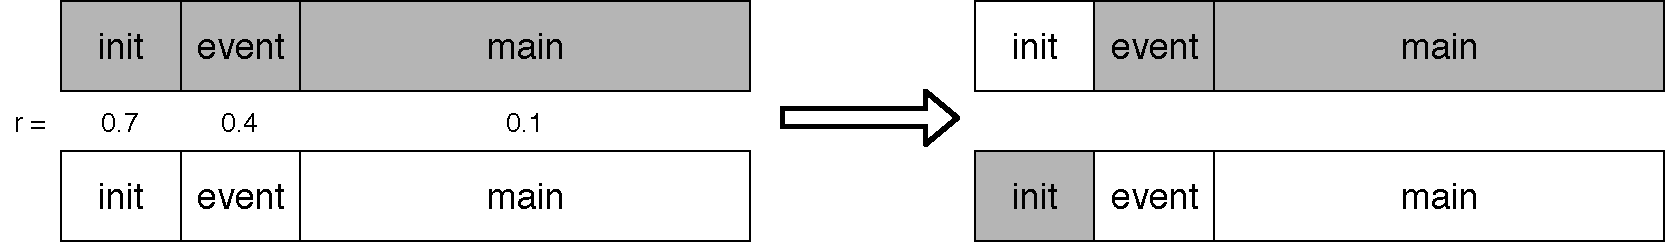
\includegraphics[width=35em]{obrazky/krizeni_podprogramu.pdf}}
    \caption{
    Vlastní uniformní křížení.
    Zde, při křížení rodičů došlo k výměně podprogramu init.
    }
    \label{fig:krizeni_podprogramu}
\end{figure}

Tento operátor se používá v experimentech se spirálovou trajektorií.
Pro experimenty s přímkovou trajektorí se používá jednobodové křížení, které pracuje na úrovni jednotlivých instrukcí.

\subsection{Mutace}
Operátor mutace je nastaven s $p_m = 1$ a vždy mutuje jen jeden gen.
Tento operátor je implementován následovně.
Náhodně se vybere jedna instrukce z genotypu.
S 20~\% pravděpodobností je tato instrukce vymazána a je nahrazena novou, náhodně vygenerovanou.
S 80~\% pravděpodobností je tato instrukce upravena a to tak, že je zde 50~\% pravděpodobnost na mutaci prvního, nebo druhého argumentu.
Mutace argumentu je implementována tak, že je hodnota zahozena a je vygenerována nová.


\subsection{Ukončovací podmínka}
Jako ukončovací podmínka byla zvoleno ukončení evoluce po provedení daného počtu generací.


\todo{zminka o implementaci programu?}

%%%%%%%%%%%%%%%%%%%%%%%%%%%%%%%%%%%%%%%%%%%%%%%%%%%%%%%%%%%%%%%%%%%%%%%%%%%%%%%%%%%%%%%%%%%%%%%%%%%%%%%%%%%%%%%%%%%%%%%%%%%%%%%%%%%%%%%%%%%%%%%%%%%%%%%%%%%%%%%%%%%%%%%%%%%
%%%%%%%%%%%%%%%%%%%%%%%%%%%%%%%%%%%%%%%%%%%%%%%%%%%%%%%%%%%%%%%%%%%%%%%%%%%%%%%%%%%%%%%%%%%%%%%%%%%%%%%%%%%%%%%%%%%%%%%%%%%%%%%%%%%%%%%%%%%%%%%%%%%%%%%%%%%%%%%%%%%%%%%%%%%
%%%%%%%%%%%%%%%%%%%%%%%%%%%%%%%%%%%%%%%%%%%%%%%%%%%%%%%%%%%%%%%%%%%%%%%%%%%%%%%%%%%%%%%%%%%%%%%%%%%%%%%%%%%%%%%%%%%%%%%%%%%%%%%%%%%%%%%%%%%%%%%%%%%%%%%%%%%%%%%%%%%%%%%%%%%

\chapter{Experimenty}
Pro účely experimentálního ověření funkčnosti použitých postupů byly navrženy 2 experimenty, které byly provedeny s každým modelem, tedy celkem 4 experimenty.

\section{Přímka}
Tento experiment měl za cíl ověřit, zda-li je použitý způsob řízení modelu funkční.
Úlohou modelu bylo pohybovat se po přímce, na které leželo 7 referenčních bodů.
V průběhu tohoto experimentu byl laďěn způsob řízení modelu a také parametry evolučního algoritmu.

\subsection{Model trojnožky}
V tomto experimentu byla použita následující nastavení:
\begin{itemize}
    \item 1000 jedinců v populaci
    \item jednobodové křížení s pravděpodobností $p_r = 0.8$
    \item ukončení běhu evoluce po 200 generacích
    \item 18 genů v genotypu
    \item pouze podprogram main
    \item délka simulace 80s
\end{itemize}

Snímek scény simulátoru pro tento experiment je na obrázku~\ref{fig:trojnozka_primka_zhora}.
\begin{figure}[h]
    \centering
    {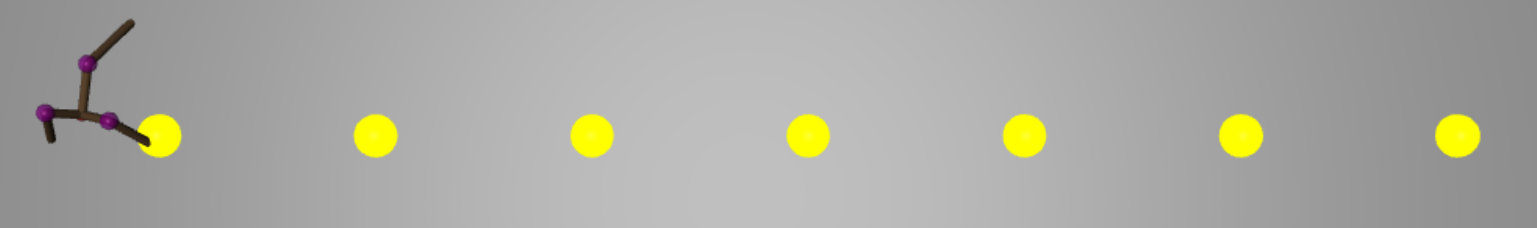
\includegraphics[width=30em]{obrazky/trojnozka_primka_zhora.png}}
    \caption{
    Scéna pro experiment s trojnožkou na přímce
    }
    \label{fig:trojnozka_primka_zhora}
\end{figure}



\subsection{Model mravence}
V tomto experimentu byla použita následující nastavení:
\begin{itemize}
    \item 400 jedinců v populaci
    \item jednobodové křížení s pravděpodobností $p_r = 0.8$
    \item ukončení běhu evoluce po 120 generacích
    \item 72 genů v genotypu
    \item pouze podprogram main
    \item délka simulace 80s
\end{itemize}

Snímek scény simulátoru pro tento experiment je na obrázku~\ref{fig:mravenec_primka_zhora}.
\begin{figure}[h]
    \centering
    {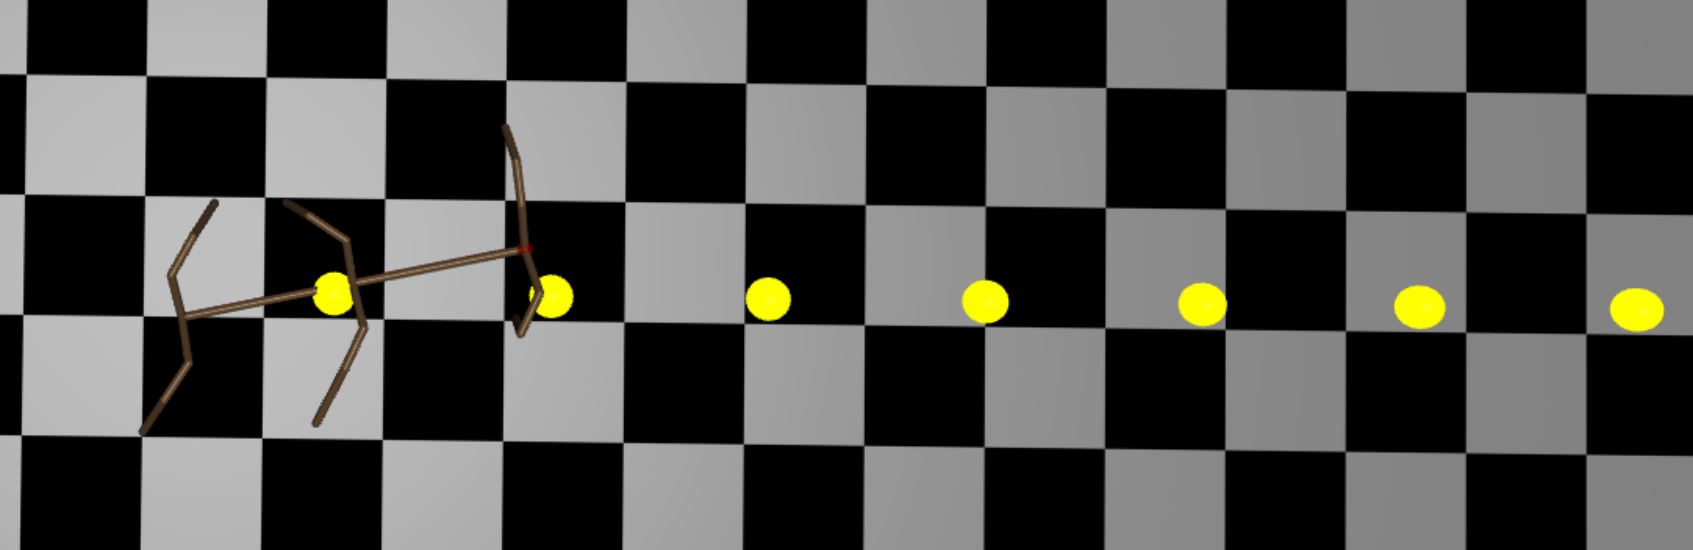
\includegraphics[width=30em]{obrazky/mravenec_primka_zhora.png}}
    \caption{
    Scéna pro experiment s mravencem na přímce
    }
    \label{fig:mravenec_primka_zhora}
\end{figure}



%%%%%%%%%%%%%%%%%%%%%%%%%%%%%%%%%%%%%%%%%%%%%%%%%%%%%%%%%%%%%%%%%%%%%%%%%%%%%%%%%%%%%%%%%%%%%%%%%%%%%%%%%%%%%%%%%%%%%%%%%%%%%%%%%%%%%%%%%%%%%%%%%%%%%%%%%%%%%%%%%%%%%%%%%%%


\section{Spirála}
Tento experiment měl za cíl ověřit, zda-li je použitý způsob řízení modelu schopný pohybu i po netriviální trajektorii, která byla definována pomocí 9 referenčních bodů.
Úlohou modelu bylo pohybovat se po spirále, na které leželo 9 referenčních bodů.
V průběhu tohoto experimentu byl laďěn systém podprogramů a vstupních informací pro program.

\subsection{Model trojnožky}
V tomto experimentu byla použita následující nastavení:
\begin{itemize}
    \item 1000 jedinců v populaci
    \item podprogramové uniformní křížení s pravděpodobností $p_r = 0.8$
    \item ukončení běhu evoluce po 300 generacích
    \item 36 genů v genotypu
    \item délka simulace 600s
\end{itemize}

Snímek scény simulátoru pro tento experiment je na obrázku~\ref{fig:trojnozka_spirala_zhora}.
\begin{figure}[h]
    \centering
    {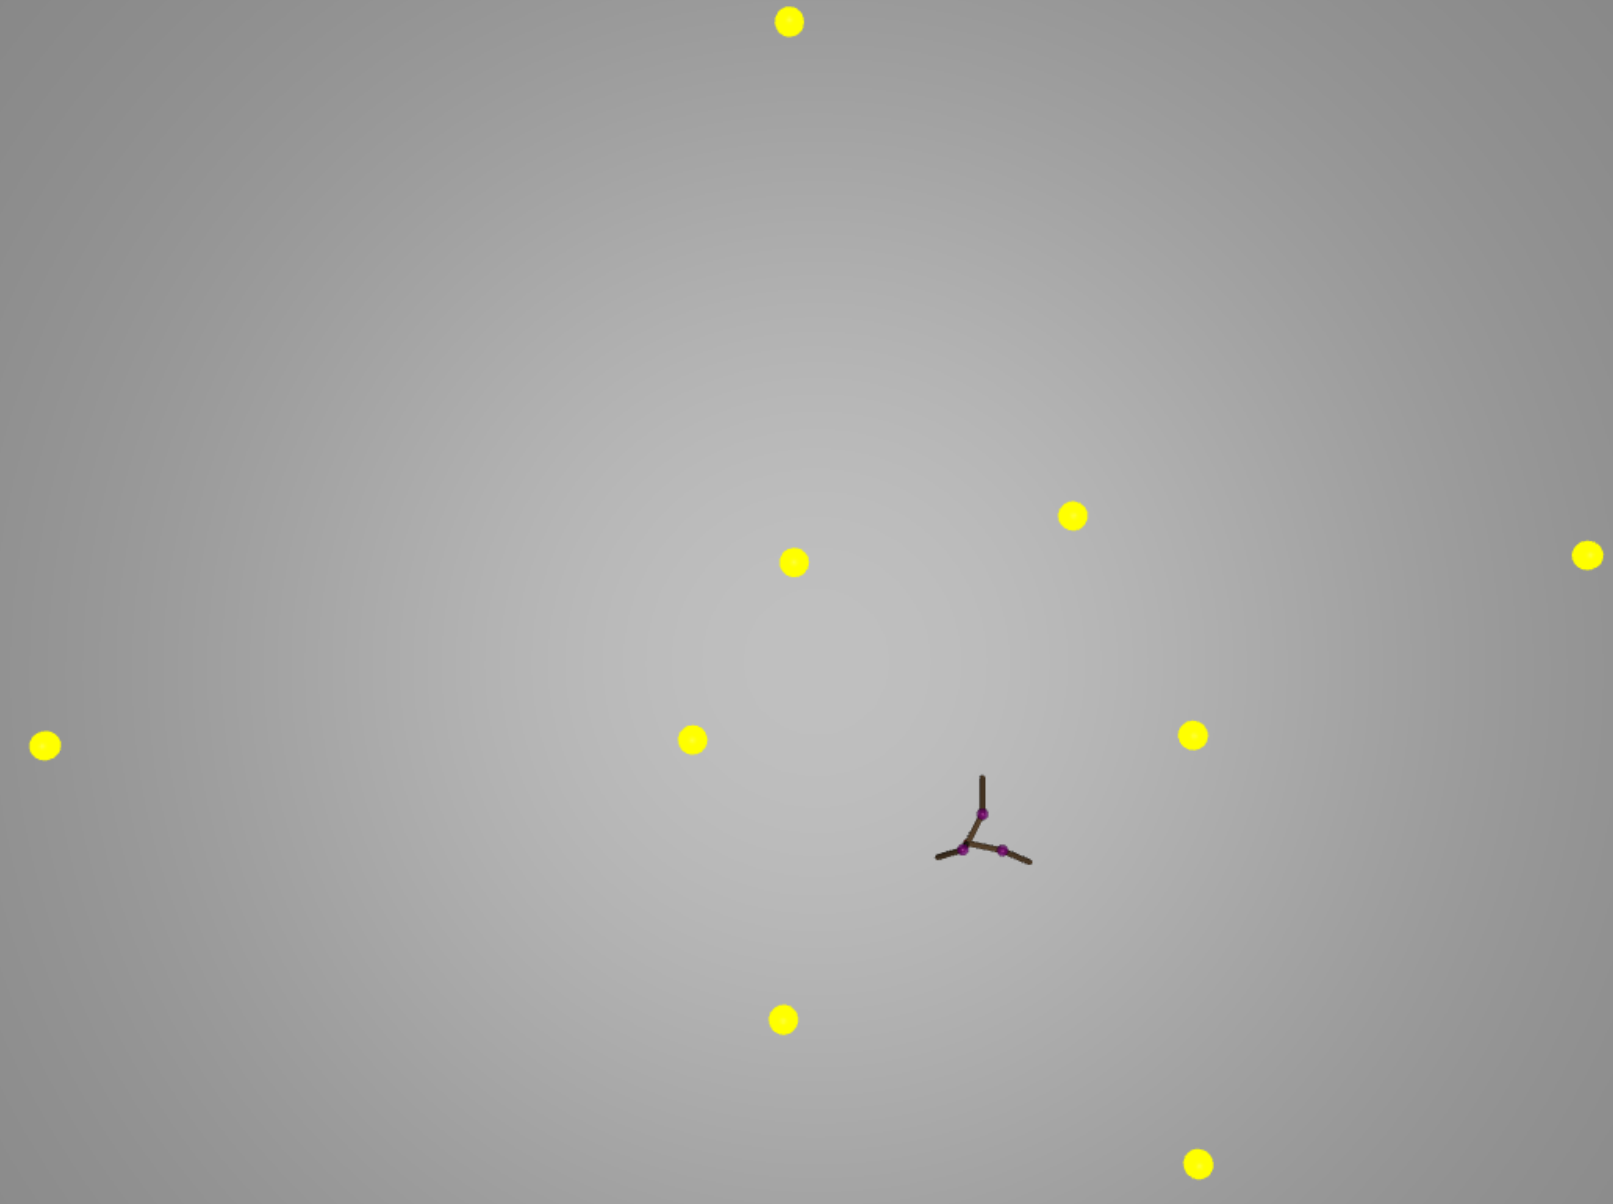
\includegraphics[width=30em]{obrazky/trojnozka_spirala_zhora.png}}
    \caption{
    Scéna pro experiment s trojnožkou na spirále
    }
    \label{fig:trojnozka_spirala_zhora}
\end{figure}

\subsection{Model mravence}

V tomto experimentu byla použita následující nastavení:
\begin{itemize}
    \item 1000 jedinců v populaci
    \item podprogramové uniformní křížení s pravděpodobností $p_r = 0.8$
    \item ukončení běhu evoluce po 300 generacích
    \item 100 genů v genotypu
    \item délka podprogramů init a event je 12 instrukcí
    \item délka simulace 600s
\end{itemize}

Snímek scény simulátoru pro tento experiment je na obrázku~\ref{fig:mravenec_spirala_zhora}.
\begin{figure}[h]
    \centering
    {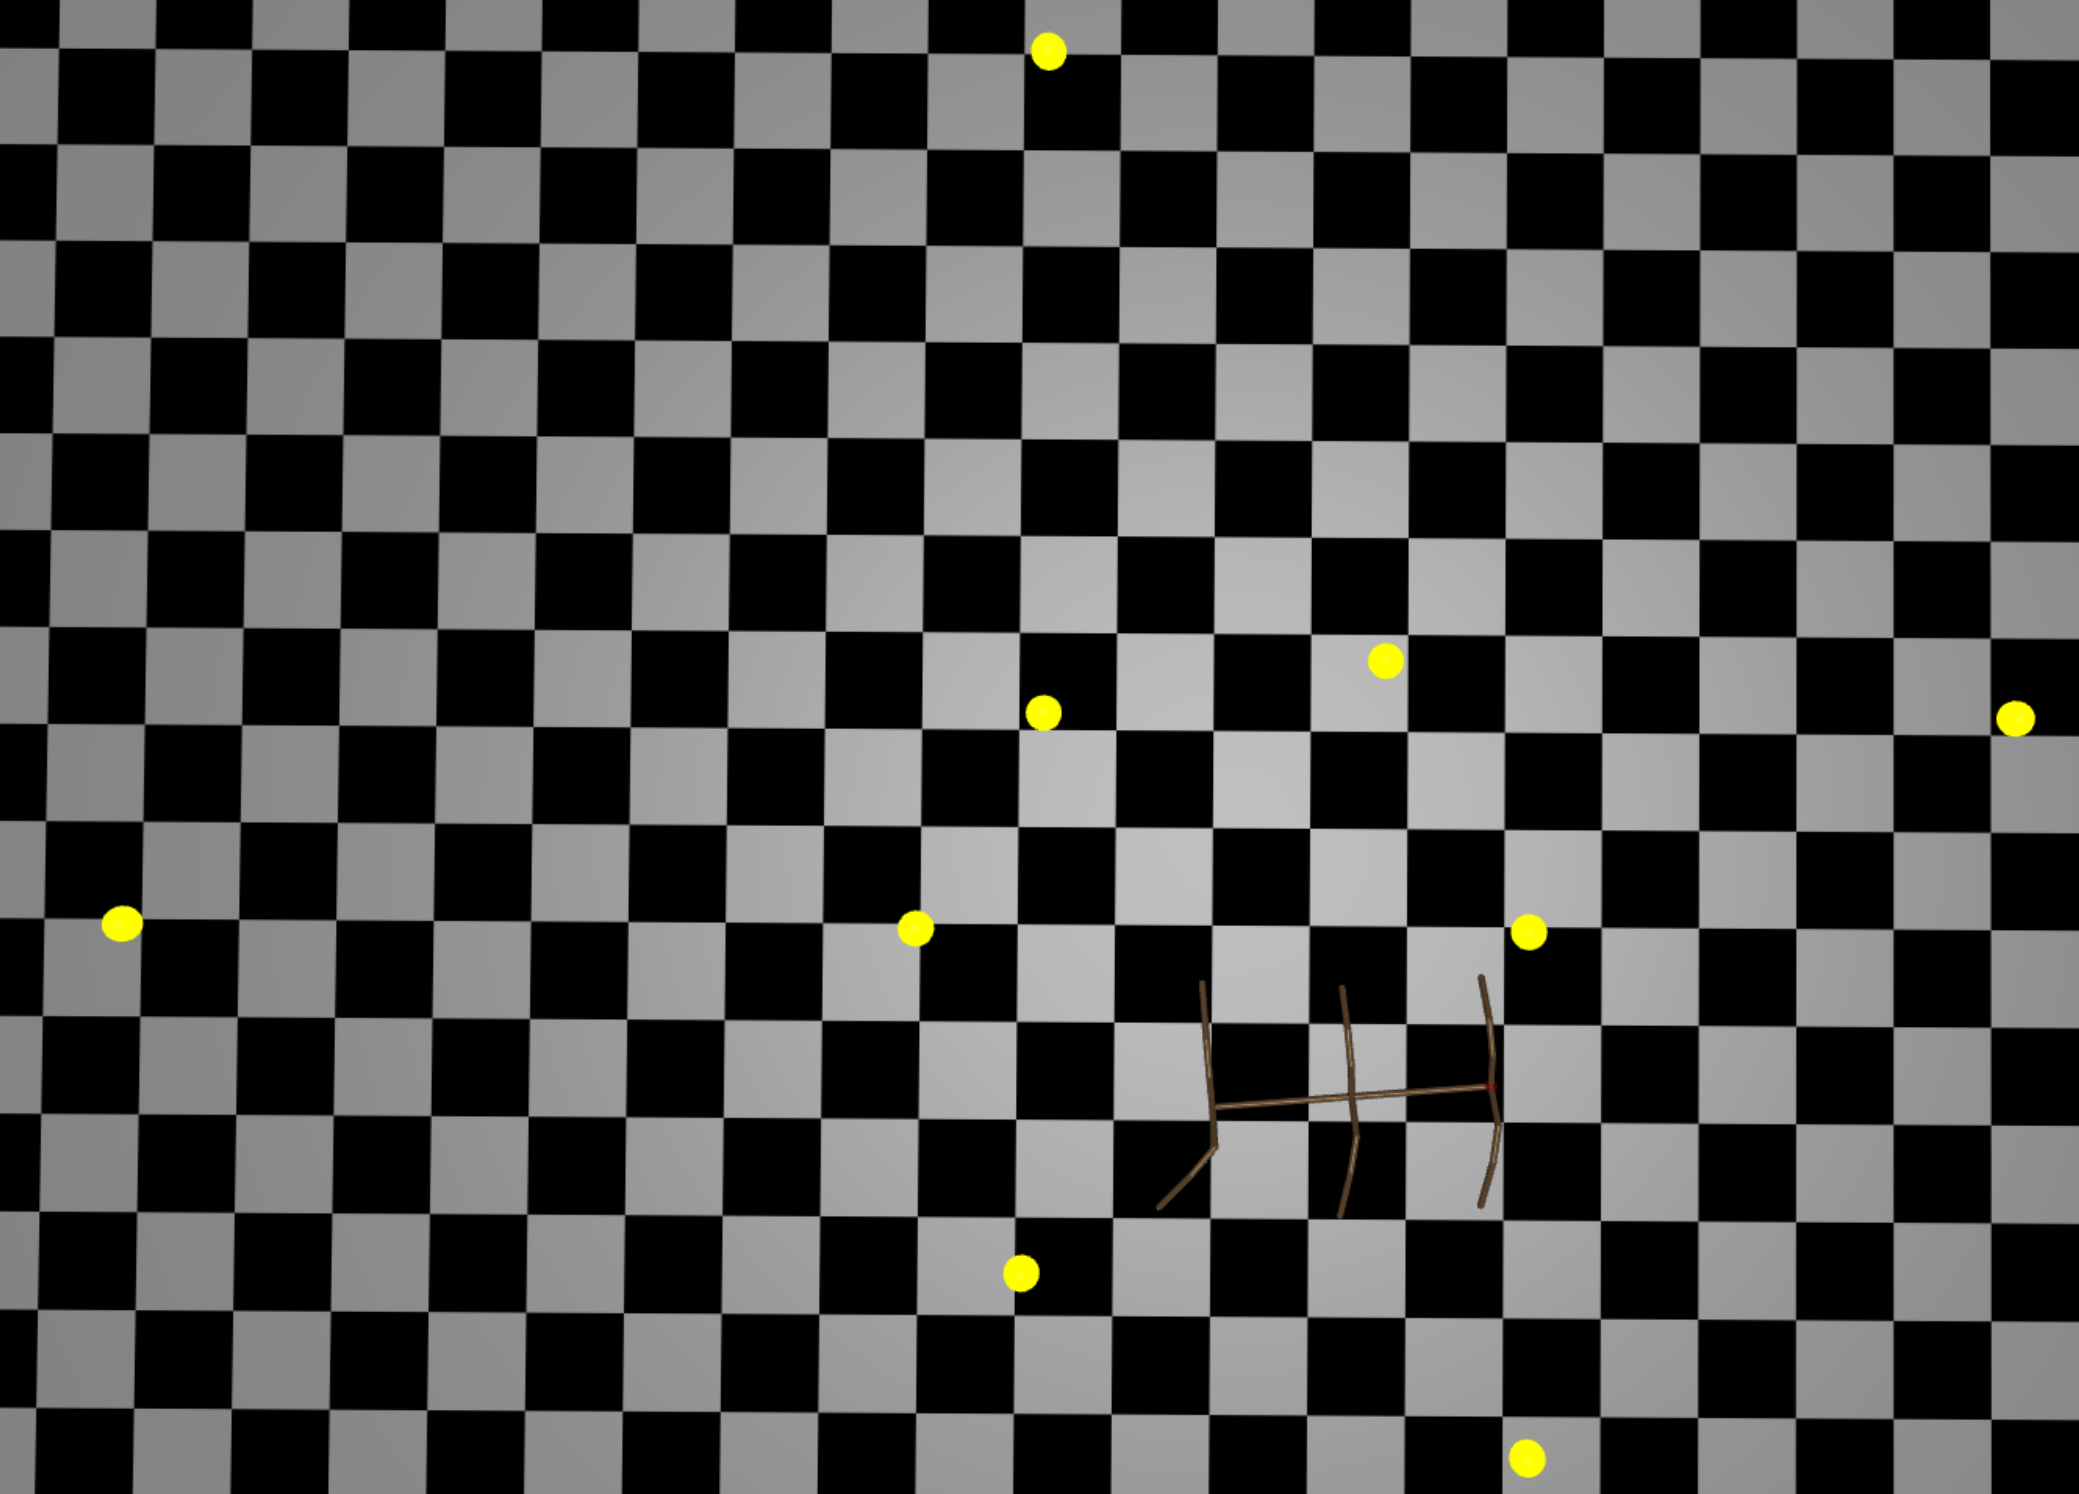
\includegraphics[width=30em]{obrazky/mravenec_spirala_zhora.png}}
    \caption{
    Scéna pro experiment s mravencem na spirále
    }
    \label{fig:mravenec_spirala_zhora}
\end{figure}


%%%%%%%%%%%%%%%%%%%%%%%%%%%%%%%%%%%%%%%%%%%%%%%%%%%%%%%%%%%%%%%%%%%%%%%%%%%%%%%%%%%%%%%%%%%%%%%%%%%%%%%%%%%%%%%%%%%%%%%%%%%%%%%%%%%%%%%%%%%%%%%%%%%%%%%%%%%%%%%%%%%%%%%%%%%
%%%%%%%%%%%%%%%%%%%%%%%%%%%%%%%%%%%%%%%%%%%%%%%%%%%%%%%%%%%%%%%%%%%%%%%%%%%%%%%%%%%%%%%%%%%%%%%%%%%%%%%%%%%%%%%%%%%%%%%%%%%%%%%%%%%%%%%%%%%%%%%%%%%%%%%%%%%%%%%%%%%%%%%%%%%
%%%%%%%%%%%%%%%%%%%%%%%%%%%%%%%%%%%%%%%%%%%%%%%%%%%%%%%%%%%%%%%%%%%%%%%%%%%%%%%%%%%%%%%%%%%%%%%%%%%%%%%%%%%%%%%%%%%%%%%%%%%%%%%%%%%%%%%%%%%%%%%%%%%%%%%%%%%%%%%%%%%%%%%%%%%


\chapter{Výsledky experimentů}
Pro každý experiment bylo provedeno 20 evolučních běhů, ze kterých byly zaznamenány fitness hodnoty všech jedinců.
Pro každý evoluční běh byly z těchto hodnot vykresleny 2 typy grafů:

\begin{itemize}
    \item vývoj maximální a průměrné fitness hodnoty jedinců v závislosti na generaci
    \item box plot fitness hodnot pro vybrané generace
\end{itemize}

Pro každý experiment byla poté vykreslena sada histogramů, které ukazují rozložení fitness hodnot jedinců napříč všemi evolučními běhy.

V této kapitole je pro každý experiment prezentován graf vývoje průměrné a maximální fitness hodnoty v populaci a také box plot fitness hodnot pro vybrané generace pro nejlepší evoluční běh.
Veškeré další grafy, které byly vygenerovány, je možné nalézt v přílohách na přiloženém médiu.

\section{Přímka}

\subsection{Model trojnožky}
\todo{mozna vypsat do tabulky pro kazdy beh: nejlepsi, prumernou fitness?}
\begin{figure}[h]
    \begin{minipage}[c]{0.48\linewidth}
        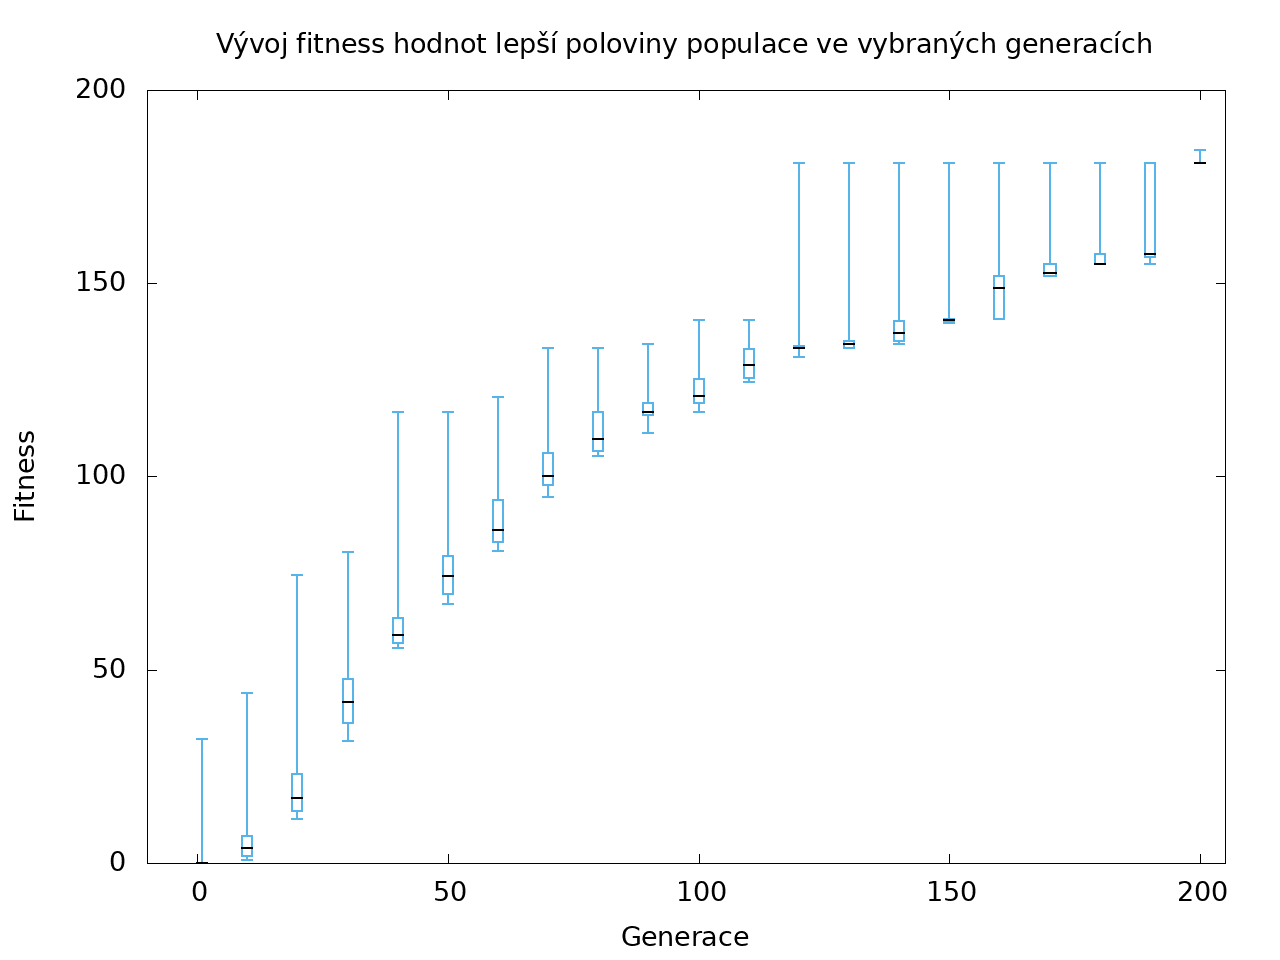
\includegraphics[width=\linewidth]{obrazky/bar_whisker_trojnozka_primka_top50.png}
        \caption{box plot fitness hodnot lepší poloviny populace pro vybrané generace}
    \end{minipage}
    \hfill
    \begin{minipage}[c]{0.48\linewidth}
        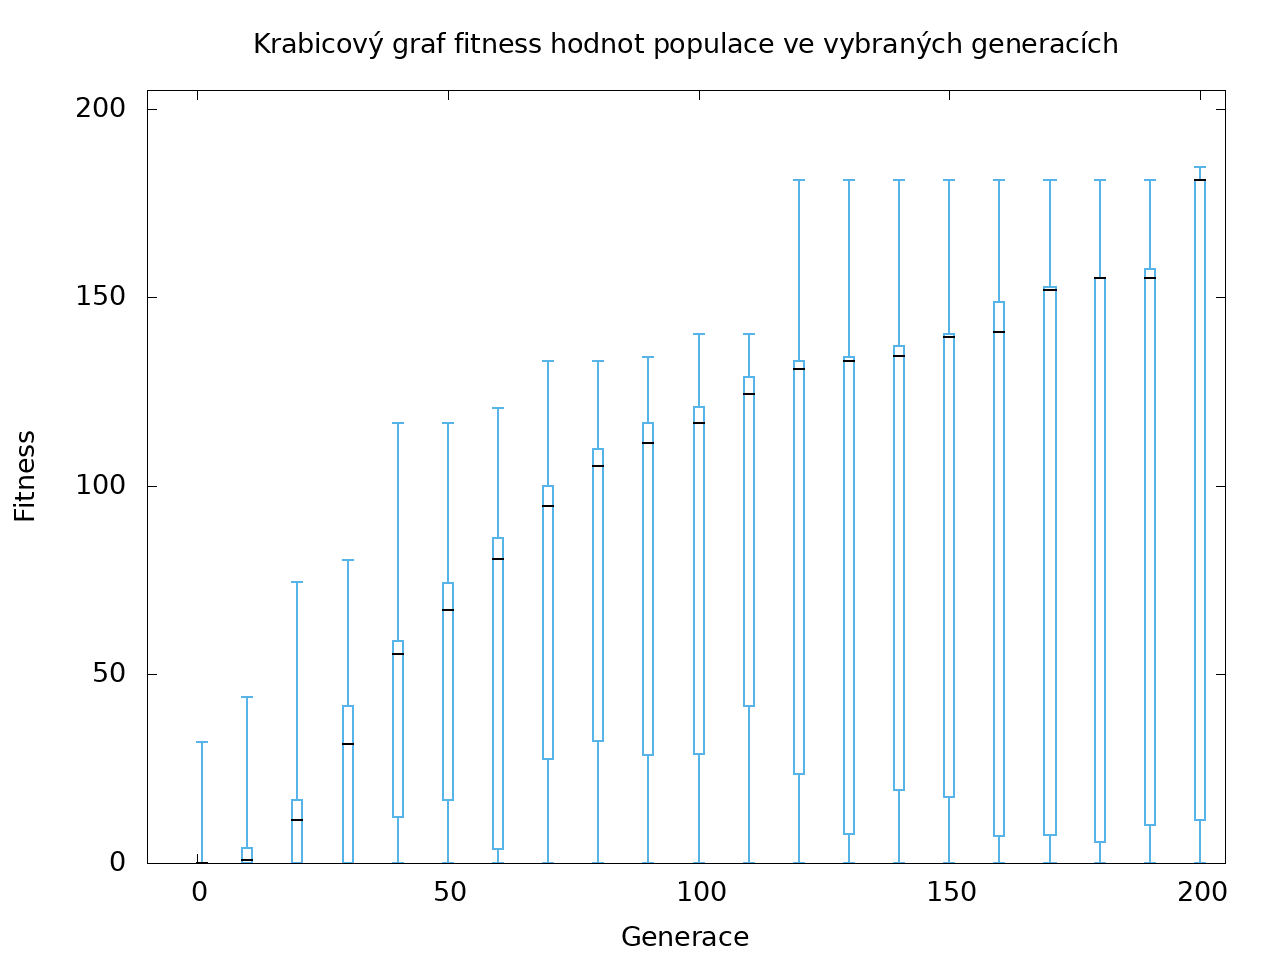
\includegraphics[width=\linewidth]{obrazky/bar_whisker_trojnozka_primka.png}
        \caption{box plot fitness hodnot populace pro vybrané generace}
    \end{minipage}
    %
\end{figure}

\begin{figure}[h]
    \centering
    {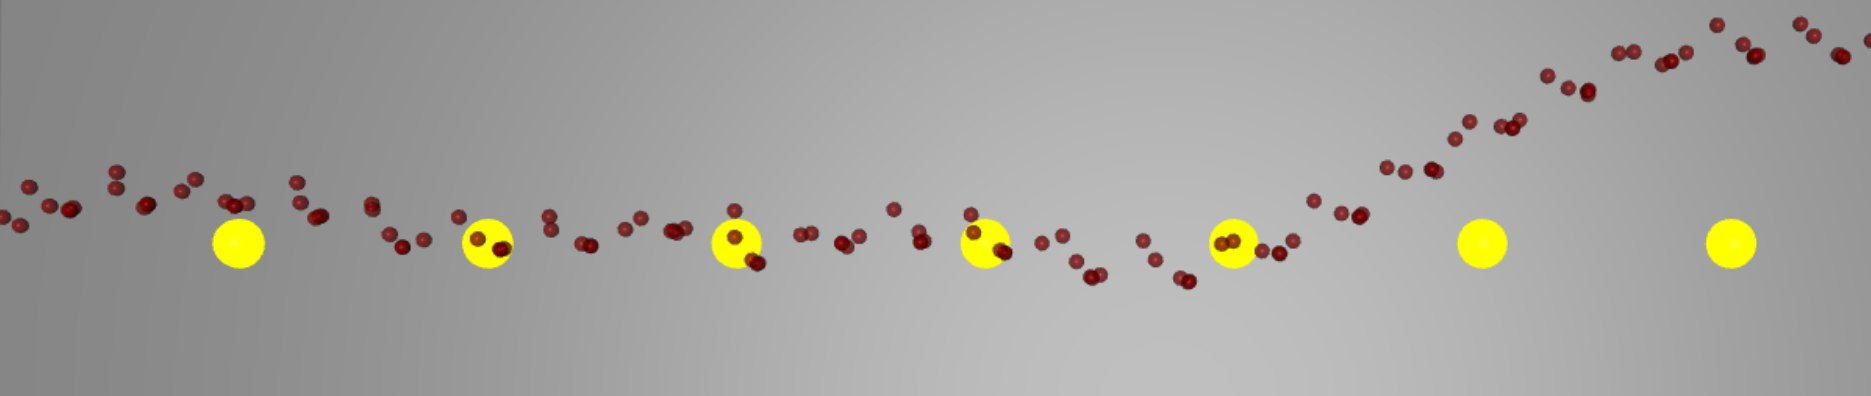
\includegraphics[width=20em]{obrazky/trojnozka_primka_zhora_nejlepsi_reseni_trajektorie.png}}
    \caption{
    Trajektorie nejlepšího rešení trojnožky na přímce
    }
    \label{fig:trojnozka_primka_zhora_nejlepsi_reseni_trajektorie}
\end{figure}



\begin{figure}[h]
    \begin{minipage}[c]{0.48\linewidth}
    {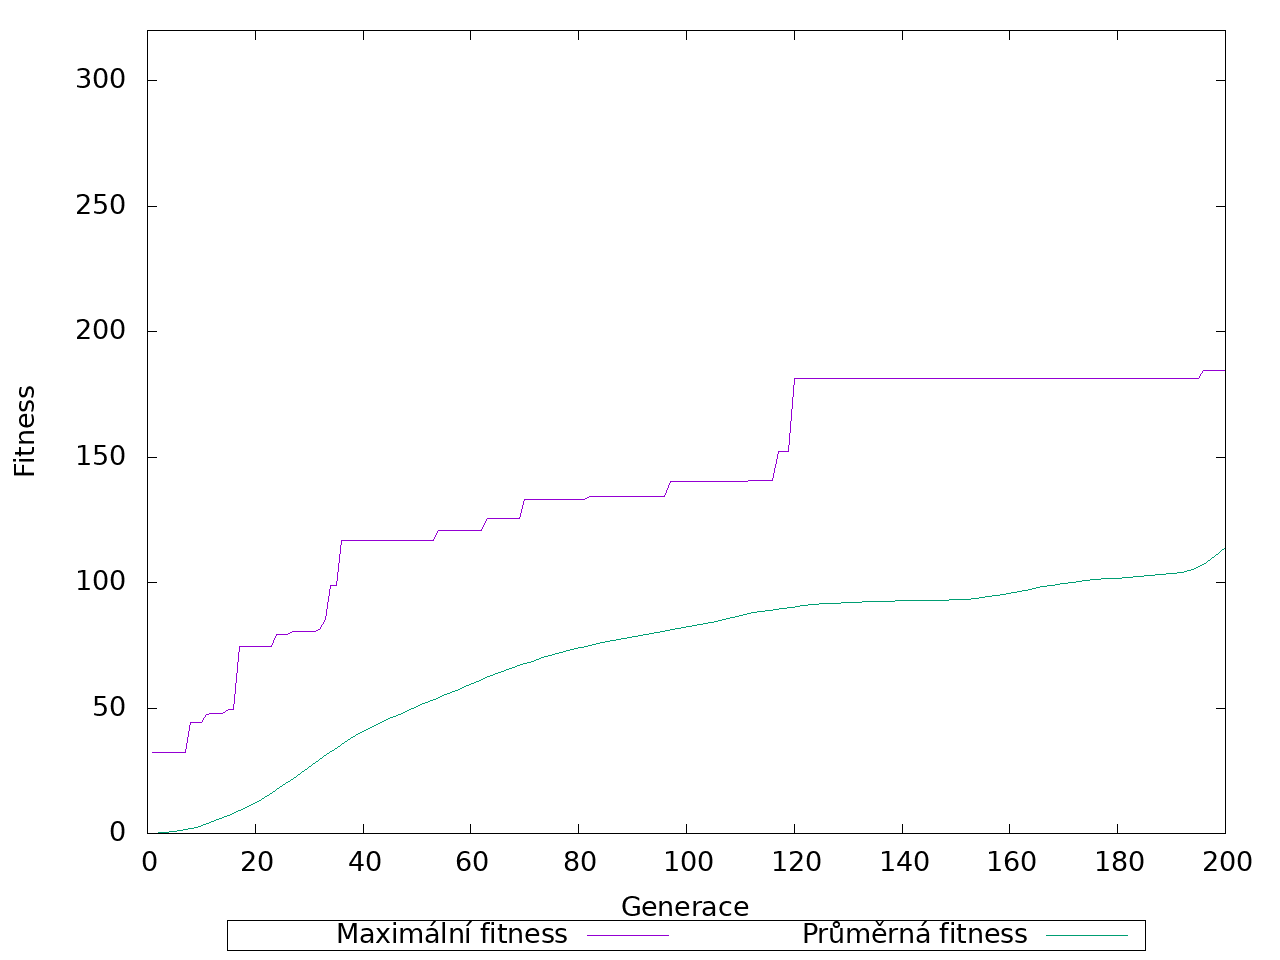
\includegraphics[width=20em]{obrazky/trojnozka_primka_fitness_prubeh.png}}
        %/home/jakub/PhpstormProjects/bp/data/bp_compute_primka_7_referenci_trojnozka_1000_jedincu_bez_rekombinace_turnaj_2_ss/2018-03-12T23:07:24+00:00/runFitnessGraph.png
        \caption{
        Nejlepší běh pro experiment s trojnožkou na přímce
        }
    \end{minipage}
    \hfill
    \begin{minipage}[c]{0.48\linewidth}
        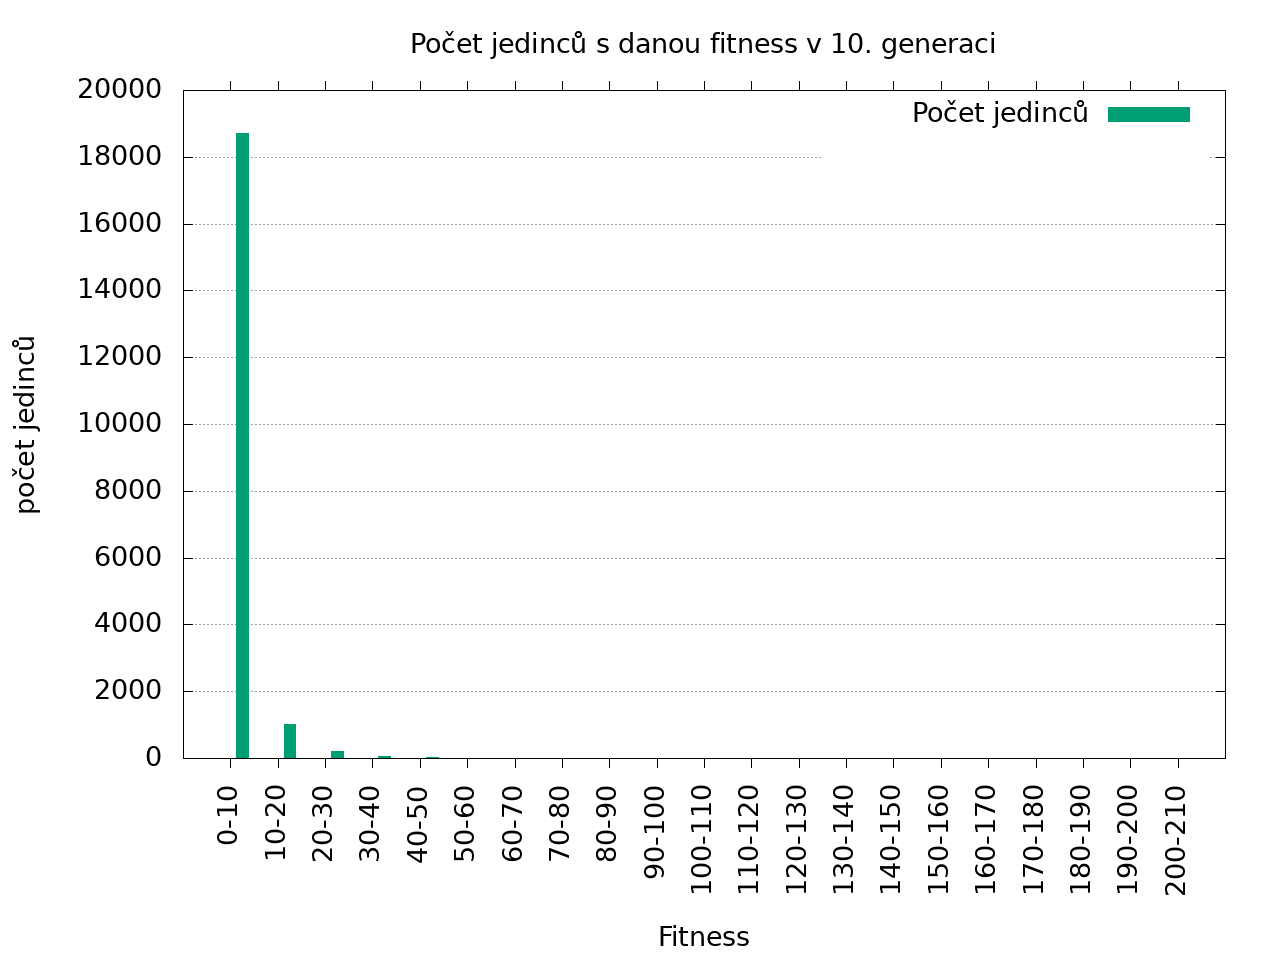
\includegraphics[width=\linewidth]{obrazky/trojnozka_primka_fitnessHistogram10.png}
        \caption{...}
    \end{minipage}
    %
\end{figure}

\begin{figure}[h]
    \begin{minipage}[c]{0.48\linewidth}
        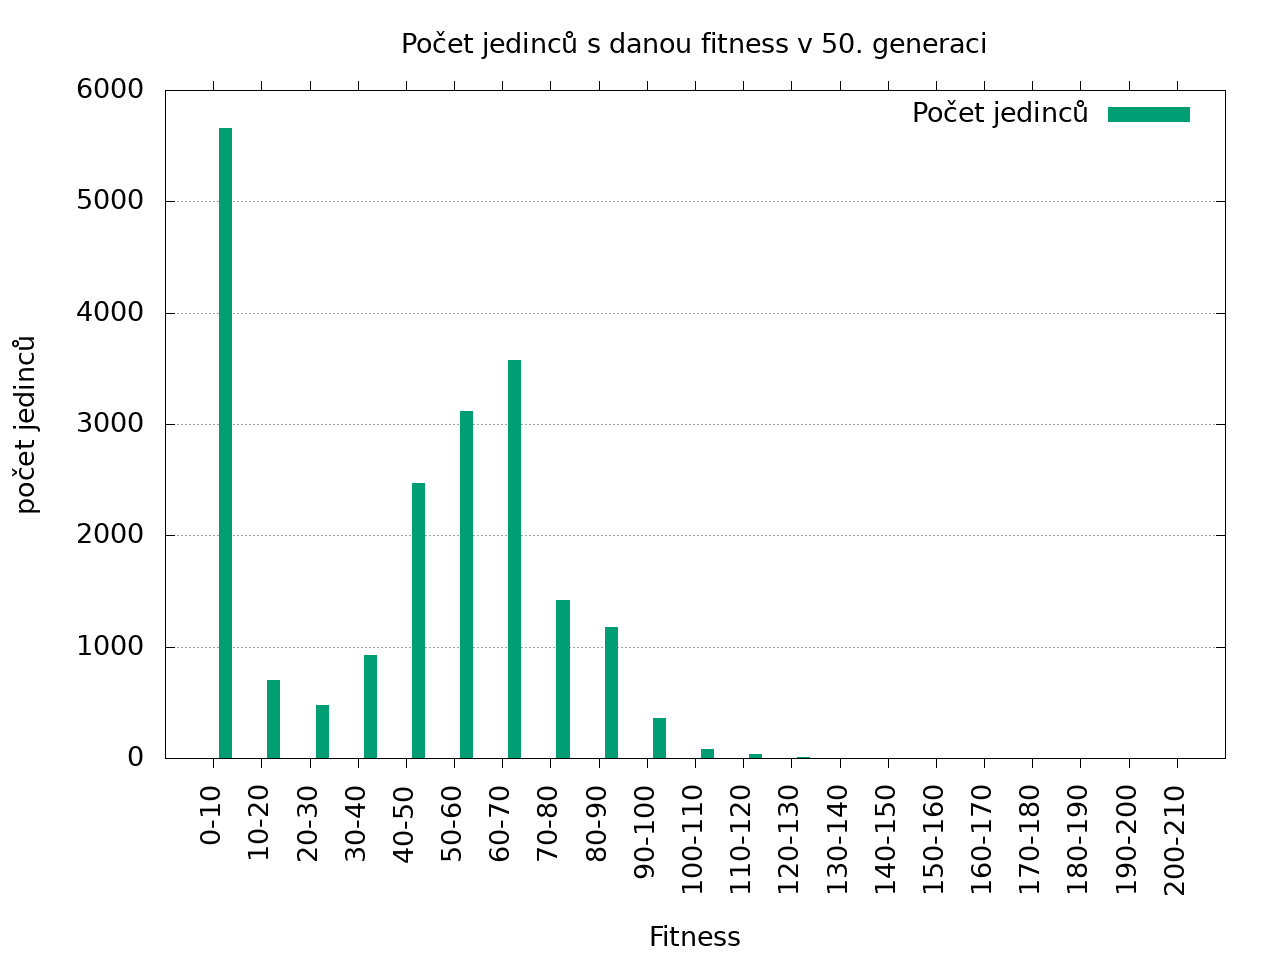
\includegraphics[width=\linewidth]{obrazky/trojnozka_primka_fitnessHistogram50.png}
        \caption{...}
    \end{minipage}
    \hfill
    \begin{minipage}[c]{0.48\linewidth}
        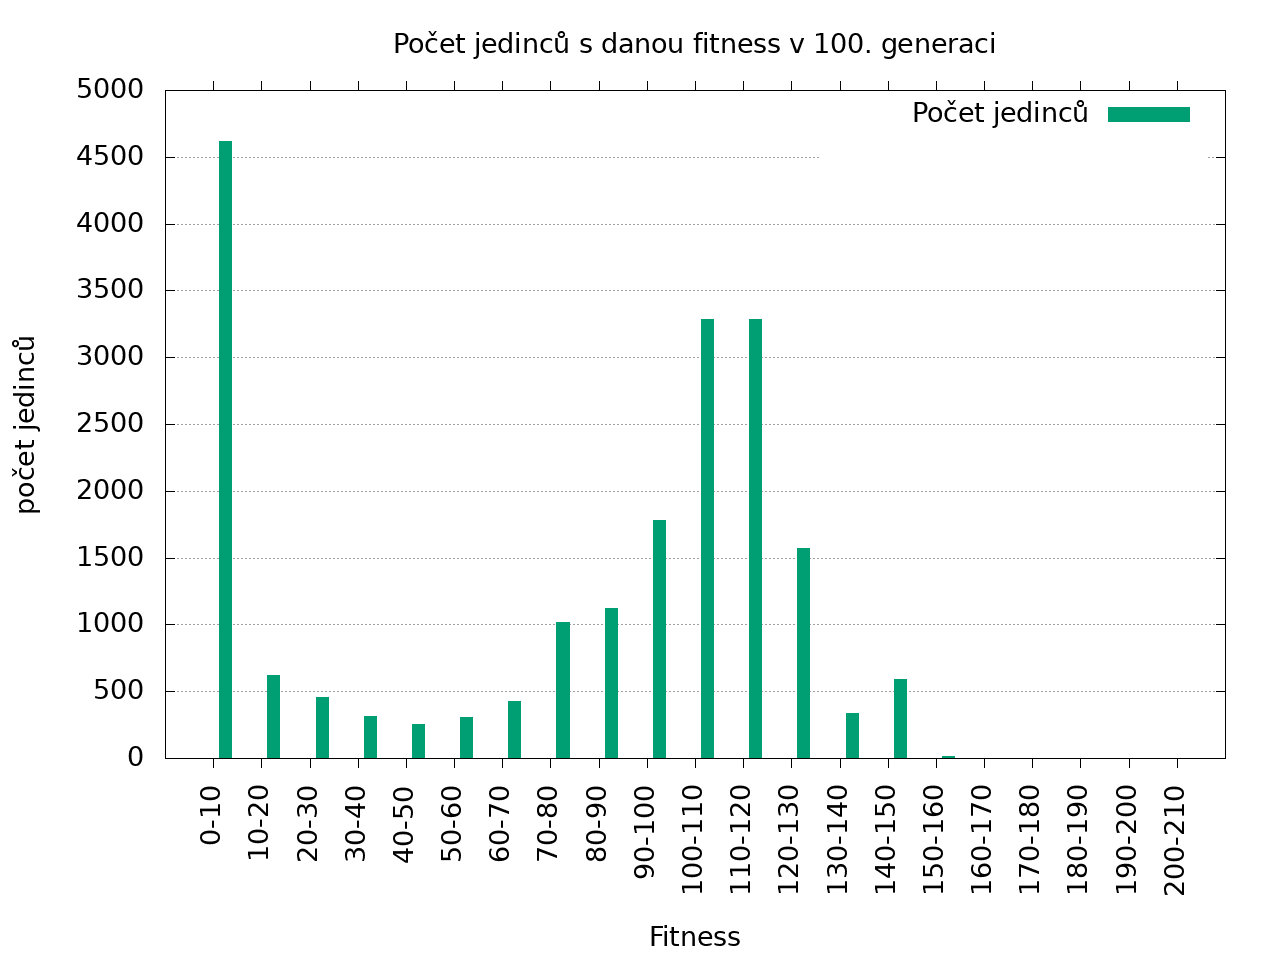
\includegraphics[width=\linewidth]{obrazky/trojnozka_primka_fitnessHistogram100.png}
        \caption{...}
    \end{minipage}
    %
\end{figure}

\begin{figure}[h]
    \begin{minipage}[c]{0.48\linewidth}
        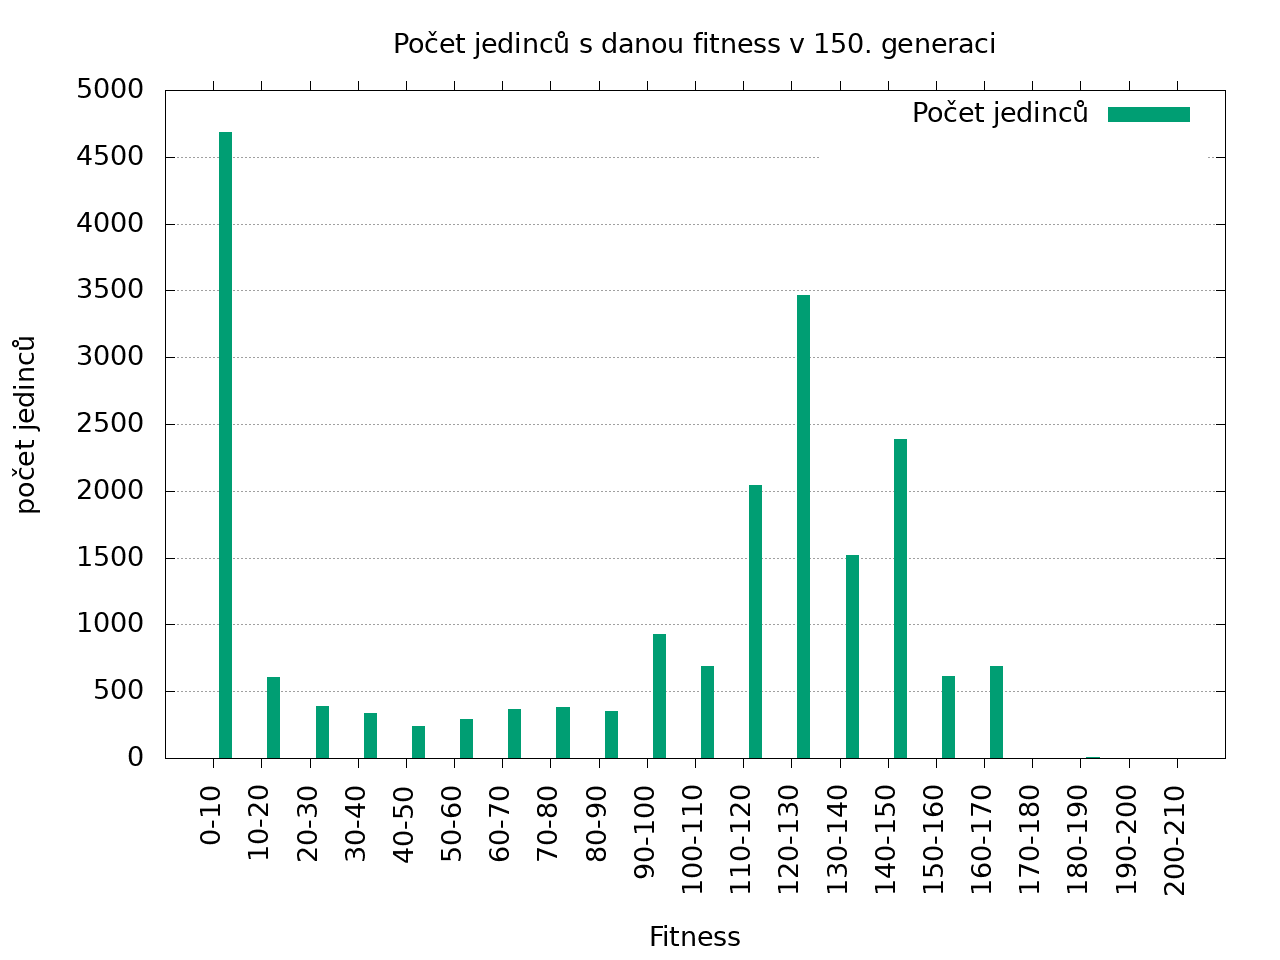
\includegraphics[width=\linewidth]{obrazky/trojnozka_primka_fitnessHistogram150.png}
        \caption{...}
    \end{minipage}
    \hfill
    \begin{minipage}[c]{0.48\linewidth}
        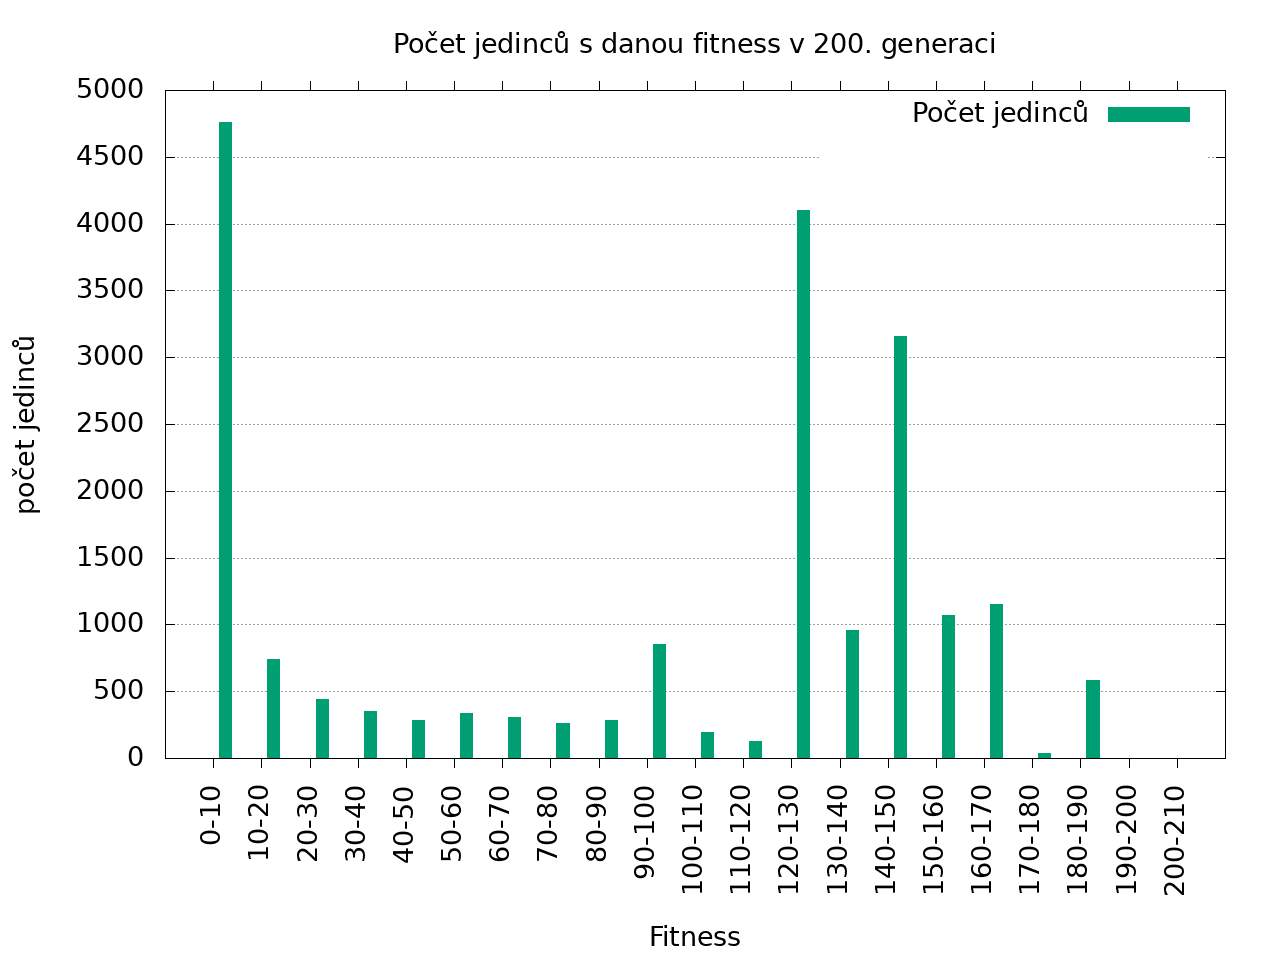
\includegraphics[width=\linewidth]{obrazky/trojnozka_primka_fitnessHistogram200.png}
        \caption{...}
    \end{minipage}
    %
\end{figure}

%donutime LaTeX vysazet vsechny obrazky, ktere dotez jeste nevysazel
\clearpage

\subsection{Model mravence}

\begin{figure}[h]
    \centering
    {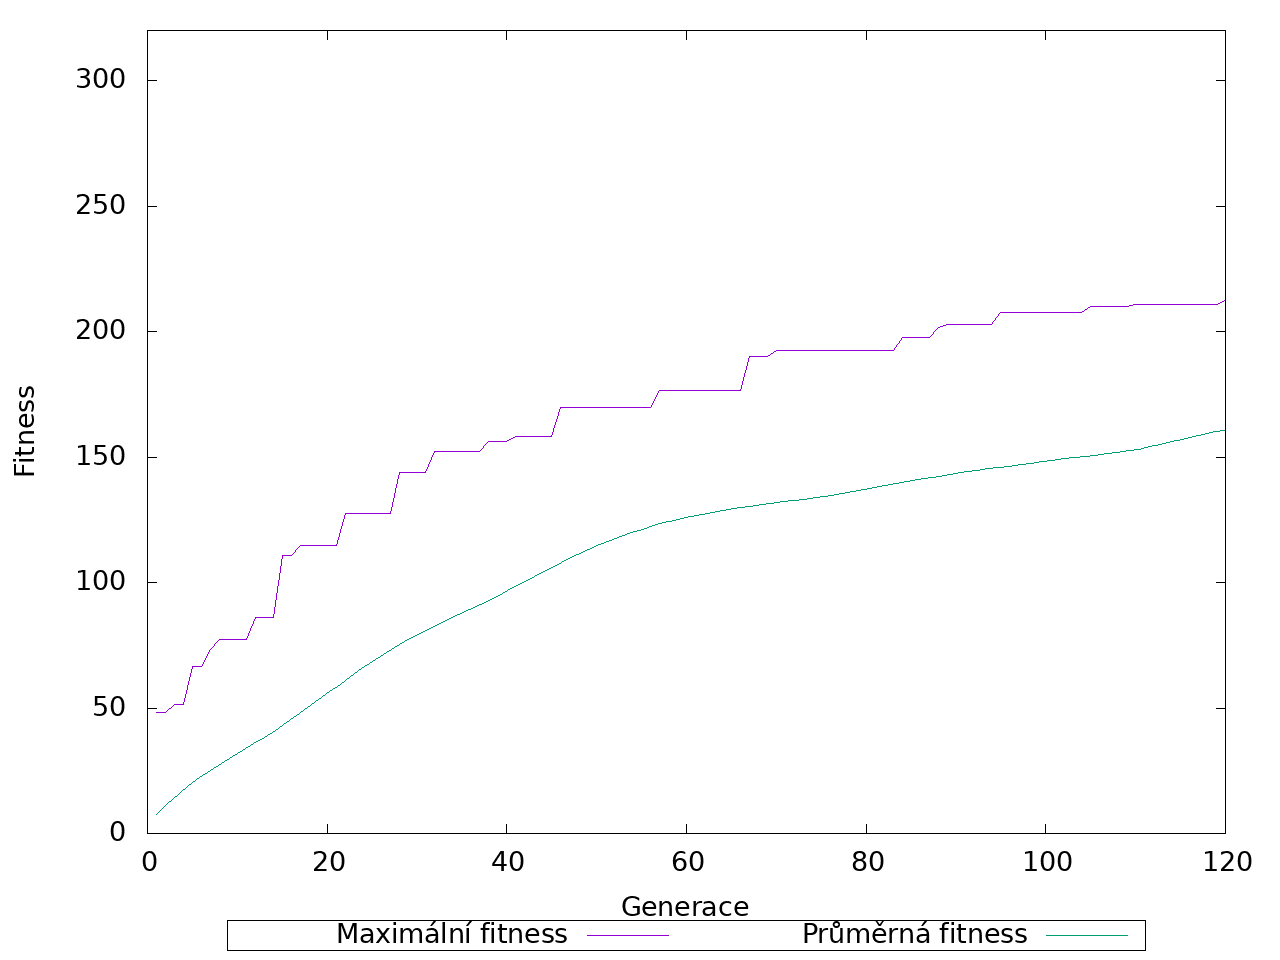
\includegraphics[width=20em]{obrazky/mravenec_primka_fitness_prubeh.png}}
    %/home/jakub/PhpstormProjects/bp/data/bp_compute_primka_7_referenci_mravenec_vstupy_2_ss/2018-05-01T01:19:54+00:00/runFitnessGraph.png
    \caption{
    Nejlepší běh pro experiment s mravencem na přímce
    }
    \label{fig:mravenec_primka_fitness_prubeh}
\end{figure}

%%%%%%%%%%%%%%%%%%%%%%%%%%%%%%%%%%%%%%%%%%%%%%%%%%%%%%%%%%%%%%%%%%%%%%%%%%%%%%%%%%%%%%%%%%%%%%%%%%%%%%%%%%%%%%%%%%%%%%%%%%%%%%%%%%%%%%%%%%%%%%%%%%%%%%%%%%%%%%%%%%%%%%%%%%%


\section{Spirála}

\subsection{Model trojnožky}
\begin{figure}[h]
    \centering
    {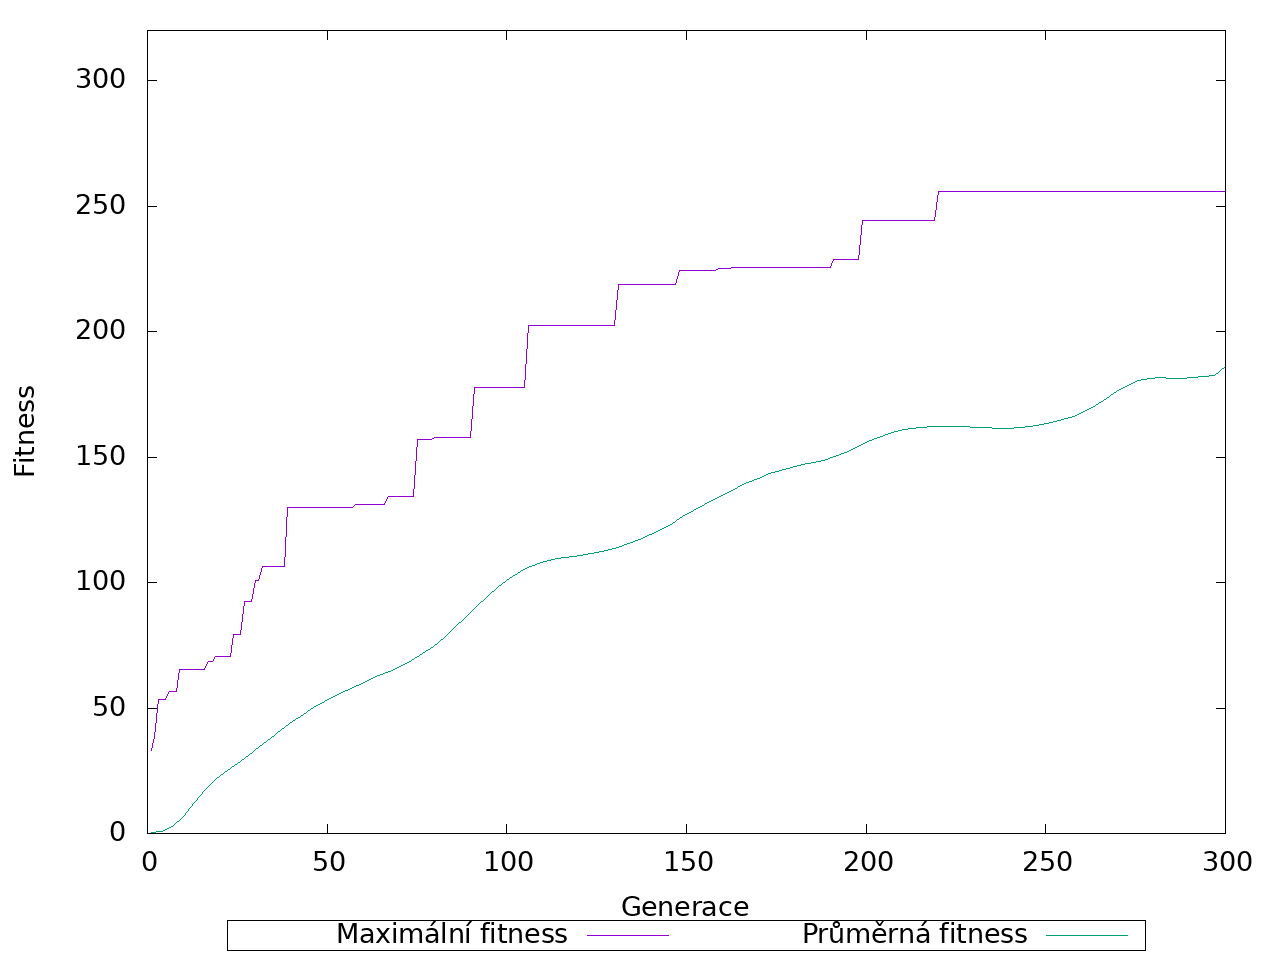
\includegraphics[width=20em]{obrazky/trojnozka_spirala_fitness_prubeh.png}}
    %/home/jakub/PhpstormProjects/bp/data/bp_compute_spirala_9_referenci_vstupy_podprogramy_2_ss/2018-03-25T17:58:49+00:00/runFitnessGraph.png
    \caption{
    Nejlepší běh pro experiment s mravencem na spirále
    }
    \label{fig:trojnozka_spirala_fitness_prubeh}
\end{figure}

\subsection{Model mravence}
\begin{figure}[h]
    \centering
    {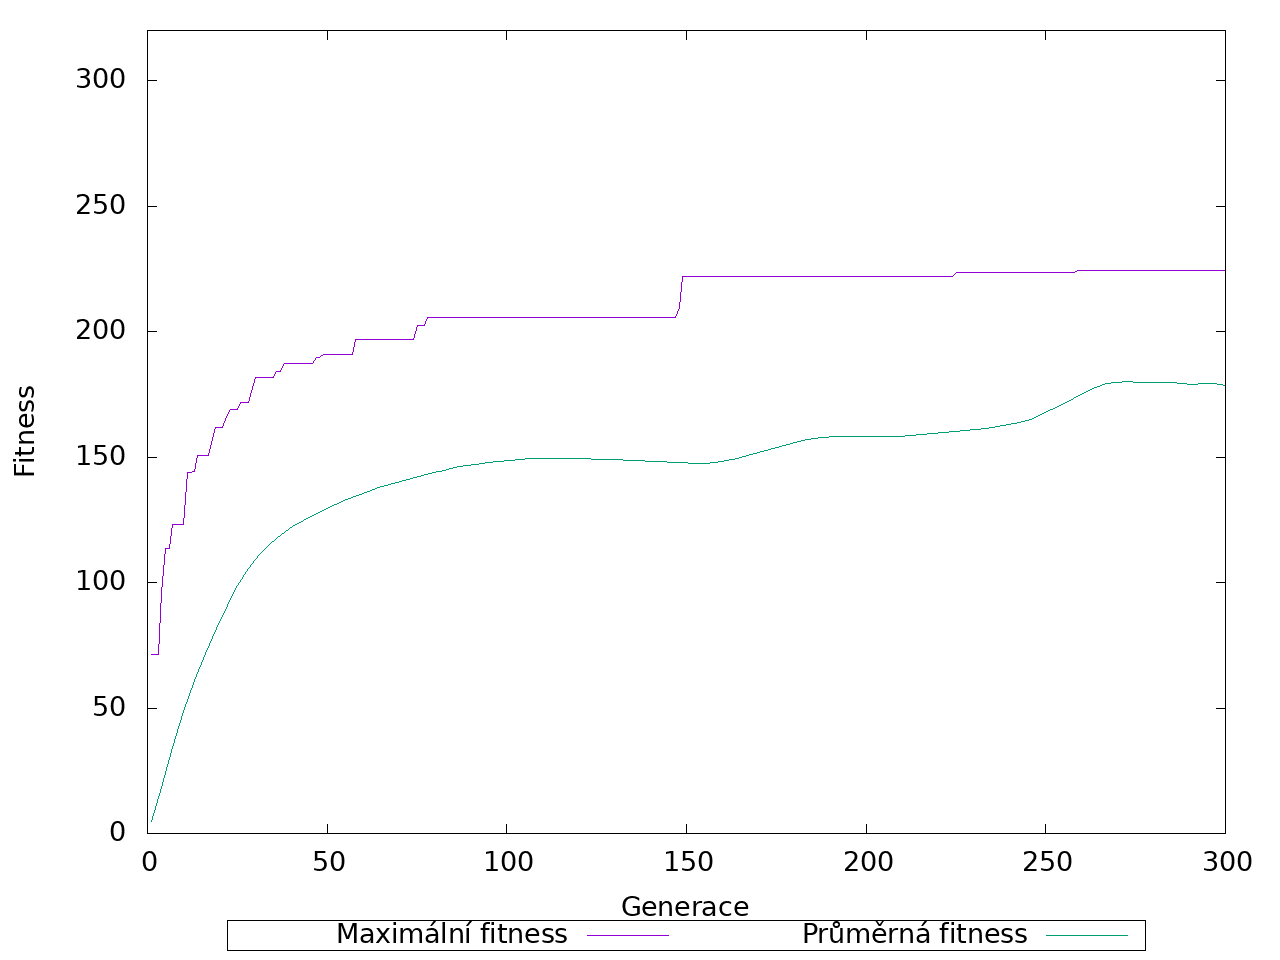
\includegraphics[width=20em]{obrazky/mravenec_spirala_fitness_prubeh.png}}
    %/home/jakub/PhpstormProjects/bp/data/bp_compute_spirala_9_referenci_mravenec_vstupy_podprogramy_2_ss/2018-03-24T13:08:39+00:00/runFitnessGraph.png
    \caption{
    Nejlepší běh pro experiment s mravencem na spirále
    }
    \label{fig:mravenec_spirala_fitness_prubeh}
\end{figure}














%%%%%%%%%%%%%%%%%%%%%%%%%%%%%%%%%%%%%%%%%%%%%%%%%%%%%%%%%%%%%%%%%%%%%%%%%%%%%%%%%%%%%%%%%%%%%%%%%%%%%%%%%%%%%%%%%%%%%%%%%%%%%%%%%%%%%%%%%%%%%%%%%%%%%%%%%%%%%%%%%%%%%%%%%%%
%%%%%%%%%%%%%%%%%%%%%%%%%%%%%%%%%%%%%%%%%%%%%%%%%%%%%%%%%%%%%%%%%%%%%%%%%%%%%%%%%%%%%%%%%%%%%%%%%%%%%%%%%%%%%%%%%%%%%%%%%%%%%%%%%%%%%%%%%%%%%%%%%%%%%%%%%%%%%%%%%%%%%%%%%%%
%%%%%%%%%%%%%%%%%%%%%%%%%%%%%%%%%%%%%%%%%%%%%%%%%%%%%%%%%%%%%%%%%%%%%%%%%%%%%%%%%%%%%%%%%%%%%%%%%%%%%%%%%%%%%%%%%%%%%%%%%%%%%%%%%%%%%%%%%%%%%%%%%%%%%%%%%%%%%%%%%%%%%%%%%%%


\chapter{Závěr}
\todo{obsah cd}
\todo{dokumentace nebo manual}

Závěrečná kapitola obsahuje zhodnocení dosažených výsledků se zvlášť vyznačeným vlastním přínosem studenta. Povinně se zde objeví i zhodnocení z pohledu dalšího vývoje projektu, student uvede náměty vycházející ze zkušeností s řešeným projektem a uvede rovněž návaznosti na právě dokončené projekty.

%=========================================================================
